\documentclass[11pt]{article}
\usepackage[]{authblk}
\usepackage{graphicx}
\usepackage{color}
\usepackage{longtable}
\usepackage{hanging}
\usepackage{indentfirst}
\usepackage{setspace}
\usepackage{verbatim}
\usepackage{upgreek}
\usepackage{framed}
\usepackage{ textcomp }
\usepackage[weather]{ifsym}
\usepackage{natbib}
\usepackage{url}
\usepackage{soul}
\usepackage{amsmath, amsfonts,amssymb,mathrsfs}
\usepackage{fancyhdr}
\usepackage[compact]{titlesec}
\usepackage[T1]{fontenc}
\usepackage{lmodern}

\setlength{\evensidemargin}{0in}
\setlength{\headheight}{0in}
\setlength{\headsep}{0in}
\setlength{\oddsidemargin}{-0.25in}
\setlength{\paperheight}{11in}
\setlength{\paperwidth}{8.5in}
\setlength{\tabcolsep}{0in}
\setlength{\textheight}{9in}
\setlength{\textwidth}{7in}
\setlength{\topmargin}{0in}
\setlength{\topskip}{0in}
\setlength{\voffset}{0in}
%\setstretch{2}
%\raggedright
\parskip = 0.15in
\pagestyle{plain}
\setlength{\parindent}{0cm}

\definecolor{citescol}{RGB}{194,101,1}
%\definecolor{citescol}{RGB}{73,0,165}
\definecolor{urlscol}{RGB}{0,150,206}
%\definecolor{urlscol}{RGB}{0,107,124}
%\definecolor{linkscol}{RGB}{187,24,0}
\definecolor{linkscol}{RGB}{149,0,207}
%\definecolor{linkscol}{RGB}{73,0,165}
\definecolor{mycol}{RGB}{25,23,191}
\definecolor{outputcol}{RGB}{34,139,34}


%\def\Fld@bordercolor{1 0 0}
%\renewcommand*{\DefaultHeightofTextMultiline}{6\baselineskip} 
%\renewcommand*{\LayoutTextField}[2]{\makebox[6em][l]{#1 }%
%  \raisebox{\baselineskip}{\raisebox{-\height}{#2}}}
%\def\LayoutChoiceField#1#2{\makebox[6em][l]{#1 }#2}

%\LayoutTextField{label}{field}

\DeclareMathAlphabet{\msfsl}{T1}{cmr}{m}{it}
\DeclareMathAlphabet{\msyf}{OMX}{pcr}{m}{it}
\newcommand{\alf}{\upalpha}
\newcommand{\hilight}[1]{\colorbox{yellow}{#1}}

\newcommand{\levelone}[1]{
\bigskip
\noindent{\LARGE{\textsc{#1}}}
\vspace {0.05in}
}

\newcommand{\leveltwo}[1]{
\bigskip
\noindent{\Large{\textit{#1}}}
\vspace {-1mm}
}

\newcommand{\descriptionhead}[1]{
\noindent{\textbf{\textit{#1}}}\\ \vspace{-7mm}
}

\newcommand{\dhead}[1]{
\noindent{\textbf{\textit{#1 --}}}
}


\newcommand{\exs}[1]{
\vspace{-4mm}
\begin{itemize}
\item #1 \\ \vspace{-8mm}
\end{itemize}
}

\newcommand{\nbo}[1]{{\color{red}{#1}}}


\newcommand{\stepbullet}{\noindent \textbullet \ }
\newcommand{\mi}[1]{\textbf{\textit{#1}}}


\newcommand{\levelthree}[1]{\textit{#1 --}}

%\newcommand{\bowtiecirclefig}{{\rlap{\rlap{{\textbf{\BigCircle}}}{\FilledTriangleLeft}}\FilledTriangleRight}}

\bibliographystyle{bib_tex/mbe}
\bibpunct[; ]{(}{)}{;}{a}{,}{;}


\usepackage[breaklinks]{hyperref}
\usepackage[all]{hypcap}
\hypersetup{colorlinks=true,linkcolor=linkscol,citecolor=citescol,urlcolor=urlscol}


\usepackage{framed}
\usepackage[]{listings}
\usepackage{fontspec}
\usepackage{placeins}
\usepackage{epstopdf}

\lstset{breaklines=true}

\definecolor{shadecolor}{RGB}{238,224,229}


\setlength{\topmargin}{-0.4in}
\setlength{\headheight}{14.5pt}
\pagestyle{fancy}

\newcommand{\taha}[1]{{\textcolor{red}{[TAH comment: #1]}}} % TAH comment

\titlespacing{\section}{0pt}{*0}{*0}
\titlespacing{\subsection}{0pt}{*0}{*0}
\titlespacing{\subsubsection}{0pt}{*0}{*0}

\titleformat{\section}
  {\normalfont\Large\bfseries\color{mycol}}
  {\thesection}{1em}{}

\titleformat{\subsection}
  {\normalfont\large\bfseries\color{mycol}}
  {\thesubsection}{1em}{}

\titleformat{\subsubsection}
  {\normalfont\bfseries\color{mycol}}
  {\thesubsection}{1em}{}

% command for MrBayes command-line step
\newcommand{\cl}[1]{{\texttt{\textbf{#1}}}}

\newcommand{\colx}[1]{{\textcolor{tcol}{#1}}}

\newcommand{\mbcl}[1]{\exs{\cl{MrBayes > {#1}}}}

\newcommand{\rbprmt}{RevBayes > } 
\newcommand{\rbcl}[1]{\exs{\cl{\rbprmt{#1}}}}
\newcommand{\rbout}[1]{\exs{\cl{\textcolor{outputcol}{#1}}}}
\newcommand{\rbdn}{{\Large \symbol{126}}} % This makes a copy/pasteable tilde
\newcommand{\rbclml}[1]{\exs{\cl{\ \ \ \ \ \ \ \ \ \ \ {#1}}}}

% text box settings
% requires compiling w/ XeLaTeX
\newfontfamily\listingsfont[Scale=1.0]{Courier New}
\lstset{basicstyle=\listingsfont, columns=texcl}
\defaultfontfeatures{Mapping=tex-text}


\makeatletter
\lst@CCPutMacro\lst@ProcessOther {"2D}{\lst@ttfamily{-{}}{-{}}}
\@empty\z@\@empty
\makeatother

\begin{document}
\renewcommand{\headrulewidth}{0.5pt}
\headsep = 20pt
\lhead{ }
\rhead{\textsc {RevBayes Tutorial --- Model Selection \& Partitioning}}

\thispagestyle{plain}
\begin{center}

\textbf{\LARGE Phylogenetic Inference using RevBayes}\\\vspace{2mm}
\textbf{\it{\Large Model Selection \& Data Partitioning}}\\\vspace{2mm}
\end{center}

\section*{Overview}

RevBayes has as a central idea that phylogenetic models, like any statistical model, are composed of smaller parts that can be decomposed and 
put back together in a modular fashion. This comes from considering phylogenetic models as \textit{probabilistic graphical models}, 
which lends flexibility and enhances the capabilities of the program. 
RevBayes implements an R-like language (complete with control statements, user-defined functions, and loops) 
that enables the user to build up phylogenetic models from simple parts (random variables, transformations, models, 
and constants of different sorts).
%RevBayes is a software program for inferring phylogenetic parameters in a Bayesian statistical framework. 
%RevBayes is ``descended'' from MrBayes \citep{huelsenbeck01c,ronquist03,huelsenbeck05,Ronquist2012}, which has been (and still is) one of the most commonly used Bayesian phylogenetic inference programs. 
%However, RevBayes is a complete rewrite and a very different approach to the engineering of the program was taken. 
%
%RevBayes uses \textit{probabilistic graphical models} for model specification and implementation \citep{hoehnaGM2014}. 
%This framework is common in the fields of statistics and machine learning to represent complex  statistical models with many parameters \citep{Gilks1994,lunn00,Jordan2004,Koller2009,Lunn2009}. 
%The graphical model tool kit allows for flexible model specification and implementation and reduces redundant code. 
%This approach to statistical inference requires a rich programming language and interface to define models and analysis details. 
%Thus, RevBayes also 

%RevBayes and the Rev language are still under active development. Thus, this tutorial comes with some caveats. First, there are many methods currently available in RevBayes, but many more that are not yet fully implemented. 
 

This tutorial demonstrates how to set up and perform an analysis that calculates Bayes factors to select among different 
partition configurations of aligned DNA sequences. 
After selecting the model that is best supported by the data, the exercise continues with basic inference of an unrooted 
tree topology and branch lengths using Markov chain Monte Carlo (MCMC). 


\bigskip
\subsection{Probabilistic Graphical Models}

RevBayes uses \textit{probabilistic graphical models} for model specification, visualization, and implementation \citep{hoehnaGM2014}. 
Graphical models are frequently used in machine learning and statistics to visually represent the conditional dependence 
structure of complex statistical models with many parameters \citep{Gilks1994,lunn00,Jordan2004,Koller2009,Lunn2009}. 
The graphical model tool kit allows for flexible model specification and implementation and reduces redundant code. 
This framework provides a set of symbols for depicting a \href{http://en.wikipedia.org/wiki/Directed_acyclic_graph}{\textit{directed acyclic graph}} (DAG). 
\citet{hoehnaGM2014} described the use of probabilistic graphical models for phylogenetics. 
The different nodes and components of a phylogenetic graphical model are shown in Figure \ref{gmnotation} \citep[Fig. 1 from][]{hoehnaGM2014}. 
\begin{figure}[h!]
\centering
\fbox{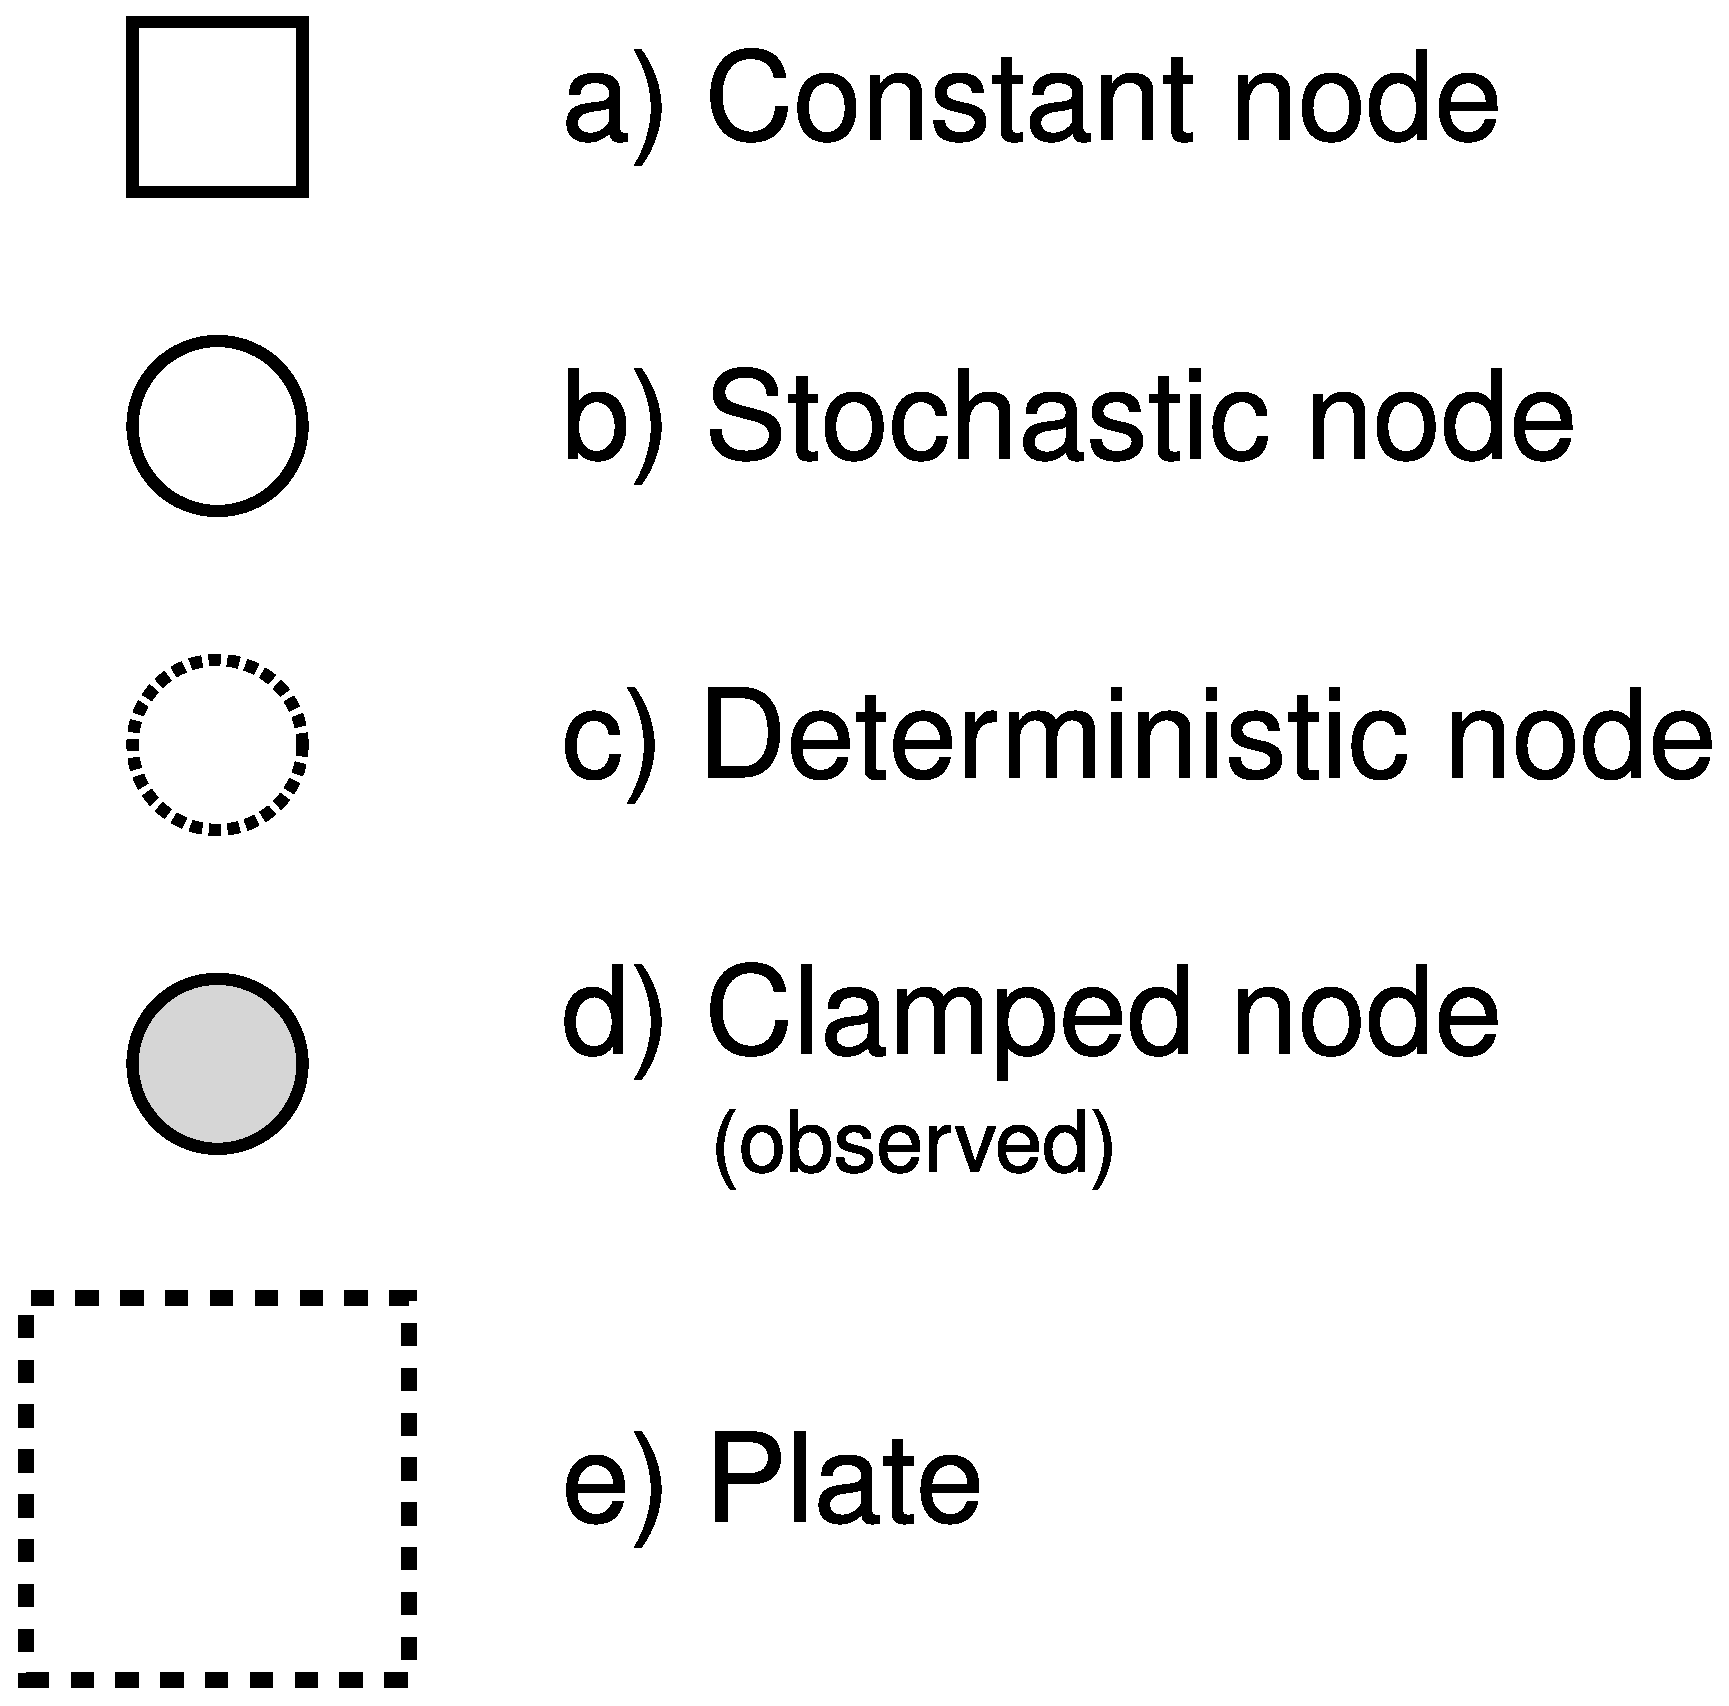
\includegraphics[width=1.8in,angle=0]{figures/GM_notation_figure.eps}}
\caption{\small The symbols for a visual representation of a graphical model. a) Solid squares represent constant nodes, 
which specify fixed-valued variables. b) Stochastic nodes are represented by solid circles. 
These variables correspond to random variables and may depend on other variables. c) Deterministic nodes (dotted circles) 
indicate variables that are determined by a specific function applied to another variable. 
They can be thought of as variable transformations. d) Observed states are placed in clamped stochastic nodes, 
represented by gray-shaded circles. e) Replication over a set of variables is indicated by enclosing the replicated nodes 
in a plate (dashed rectangle). [Replicated from Fig.~1 in \citet{hoehnaGM2014}.]}
\label{gmnotation}
\end{figure}

To represent the DAG, nodes are connected with arrows indicating dependency. 
A simple, albeit abstract, graphical model is shown in Figure \ref{simpleGM}. 
In this model, we observe a set of states for parameter $x$. 
We assume that the values of $x$ are samples from a lognormal distribution with a location parameter (log mean) 
$\mu$ and a standard deviation $\sigma$. 
It is more straightforward to model our uncertainty in the expectation of a lognormal distribution, rather than $\mu$, 
thus we place a gamma distribution on the mean $M$. This gamma hyperprior has two parameters that we specify with fixed 
values (constant nodes): the shape $\alpha$ and rate $\beta$. 
With this prior density, the variable $M$ is a stochastic node.
The standard deviation, $\sigma$, is also a stochastic node with an exponential prior density with rate parameter $\lambda$.
For any value of $M$ and any value of $\sigma$ we can compute the deterministic variable $\mu$ using the formula 
$\mu = \ln(M) - \frac{\sigma^2}{2}$. 
This formula is known from using simple algebra on the equation for the mean of any \href{http://en.wikipedia.org/wiki/Log-normal_distribution}{lognormal distribution}.
With this model structure, we can then calculate the probability of the data conditional on the model (the likelihood): 
$\mathbb{P}(\boldsymbol{x} \mid \mu, \sigma)$. With this, we can get the posterior probability using Bayes' theorem:
$$\mathbb{P}(M,\sigma \mid \boldsymbol{x}, \alpha, \beta, \lambda) = \frac{\mathbb{P}(\boldsymbol{x} \mid \mu, \sigma) \mathbb{P}(M \mid \alpha,\beta) \mathbb{P}(\sigma \mid \lambda)}{\mathbb{P}(\boldsymbol{x})}.$$
\begin{figure}[h!]
\centering
\fbox{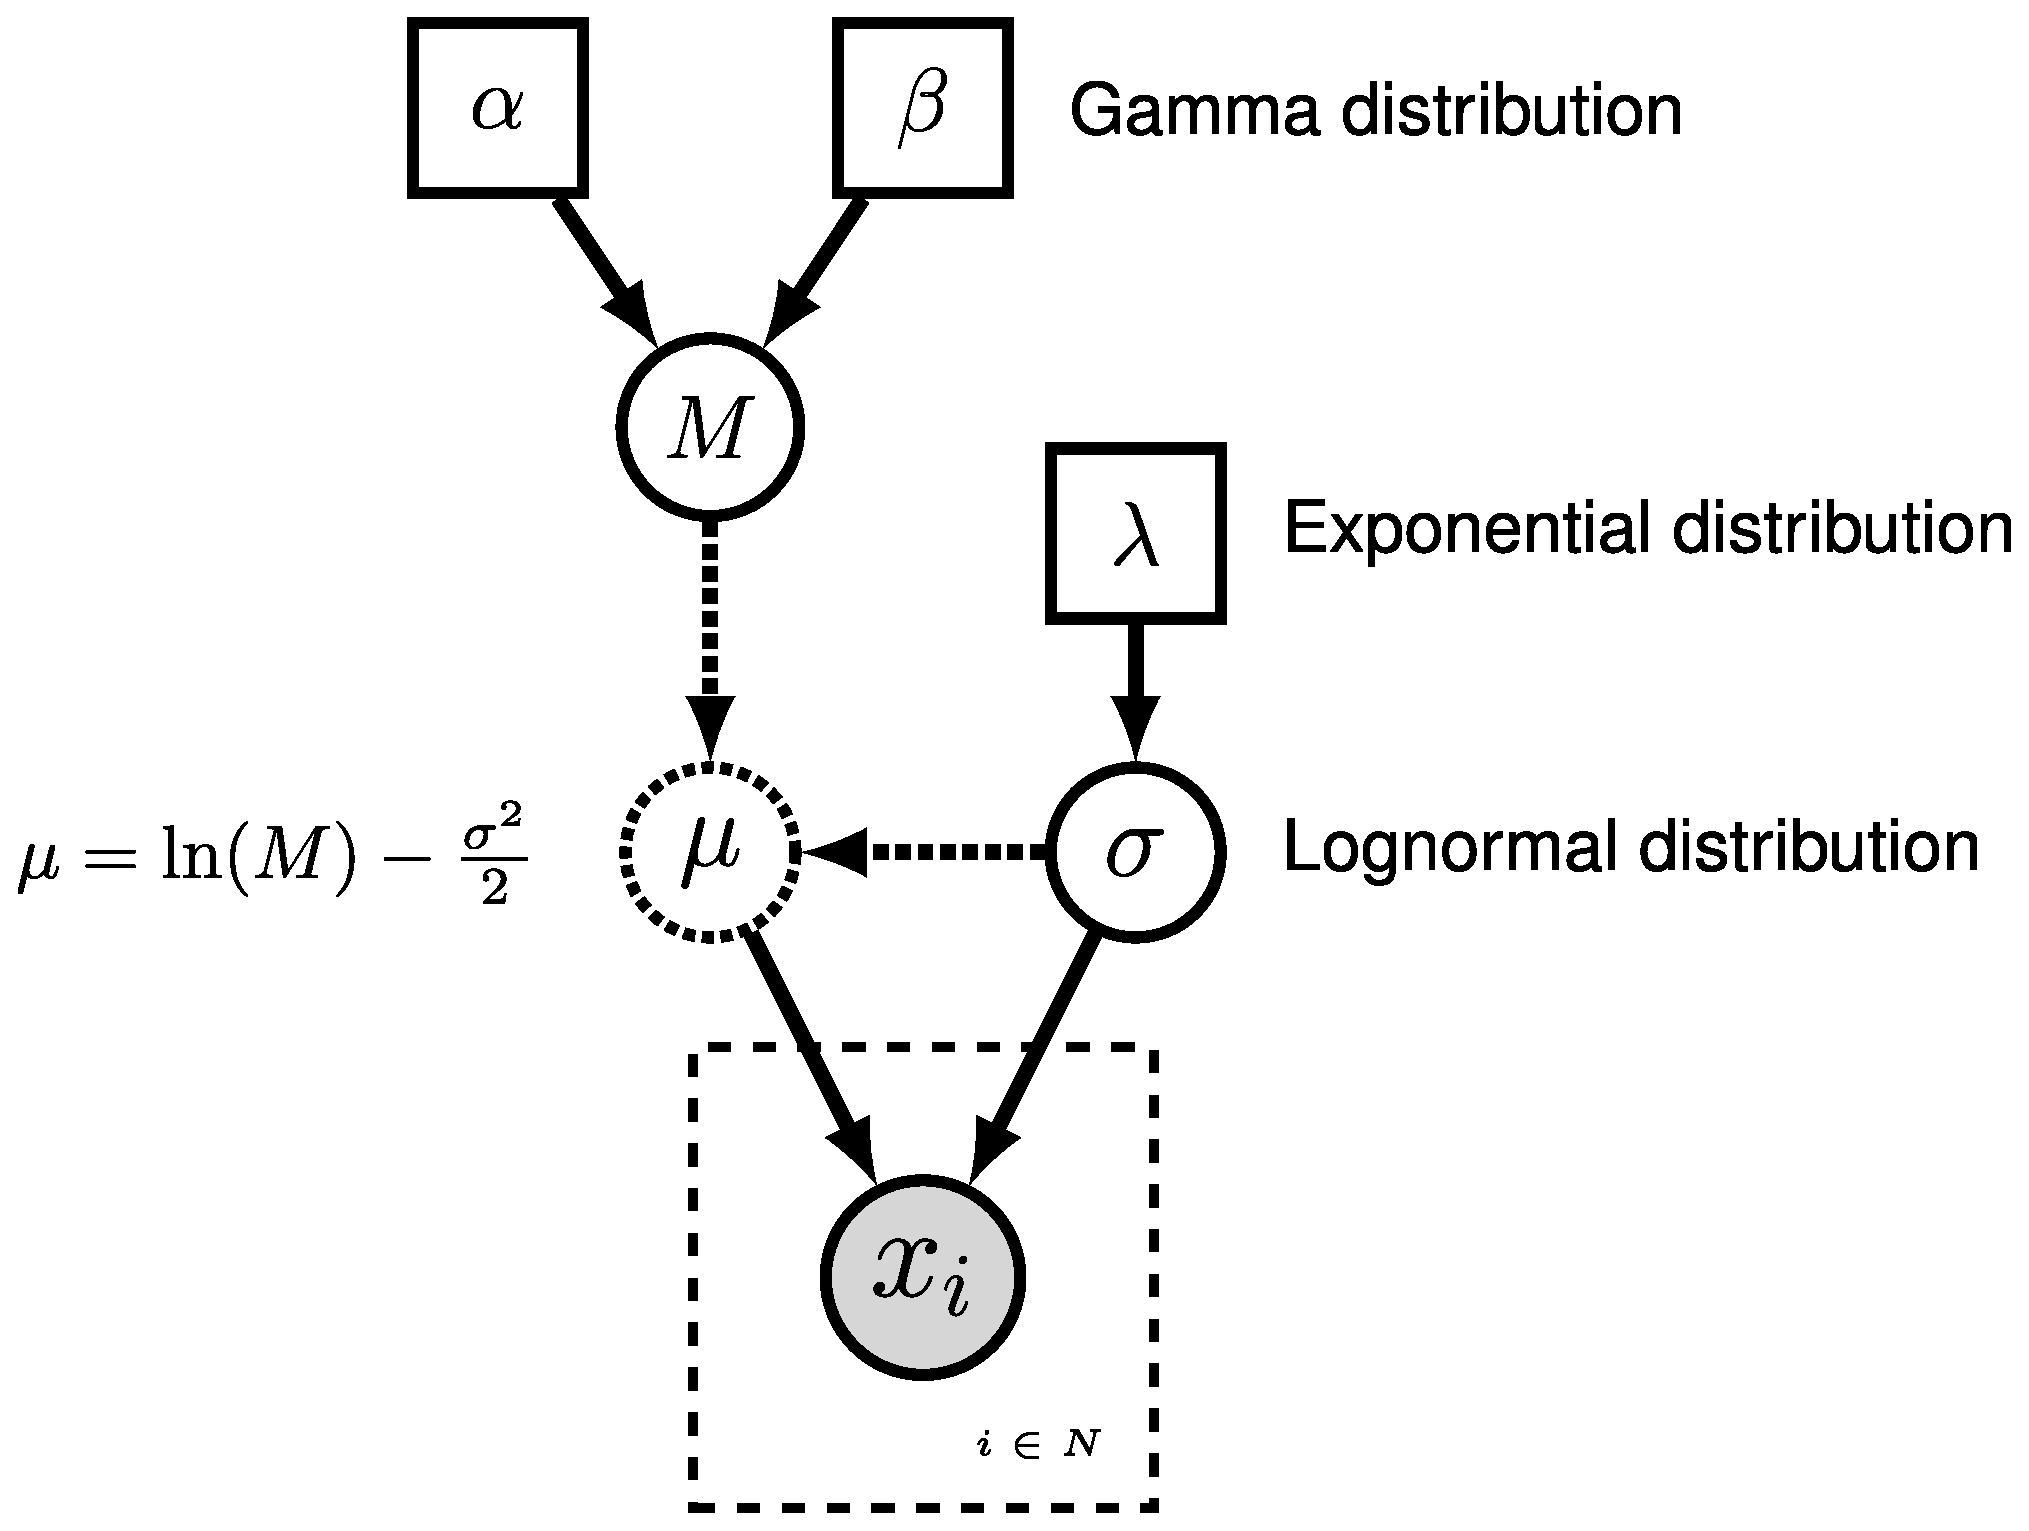
\includegraphics[width=2.5in,angle=0]{figures/simple_GM.eps}}
\caption{\small Graphical model representation of a simple lognormal model. A total of $N$ states of parameter $x$ are observed and occupy a clamped node. This parameter is log-normally 
distributed with parameters $\mu$ and $\sigma$ (log mean and standard deviation, respectively). The parameter $\mu$ is a 
deterministic node that is calculated from the stochastic nodes $M$ (the mean of the distribution) and $\sigma$. 
Dotted arrows indicate deterministic functions and are used to connect deterministic nodes to their parent variables. 
A gamma distribution is applied as a hyper prior on $M$ with constant nodes for the shape $\alpha$ and rate $\beta$. 
The stochastic variable $\sigma$ is exponentially distributed with fixed value for the rate $\lambda$.}
\label{simpleGM}
\end{figure}

For phylogenetic graphical model representations, \citet{hoehnaGM2014} introduced a new element called the \textit{tree plate}. 
This is a convenience for visualization because, although a phylogenetic tree is a graphical model, the complexity becomes intractable for large trees. 
Thus, the tree plate depicts replication over a given topology. 
The full graphical model with the unrooted tree plate for the GTR$+\Gamma$ model used in this tutorial is shown in Figure \ref{gtrgmfig}. Note that even unrooted analyses arbitrarily assign a root node to orient the tree.
\begin{figure}[h!]
\centering
\fbox{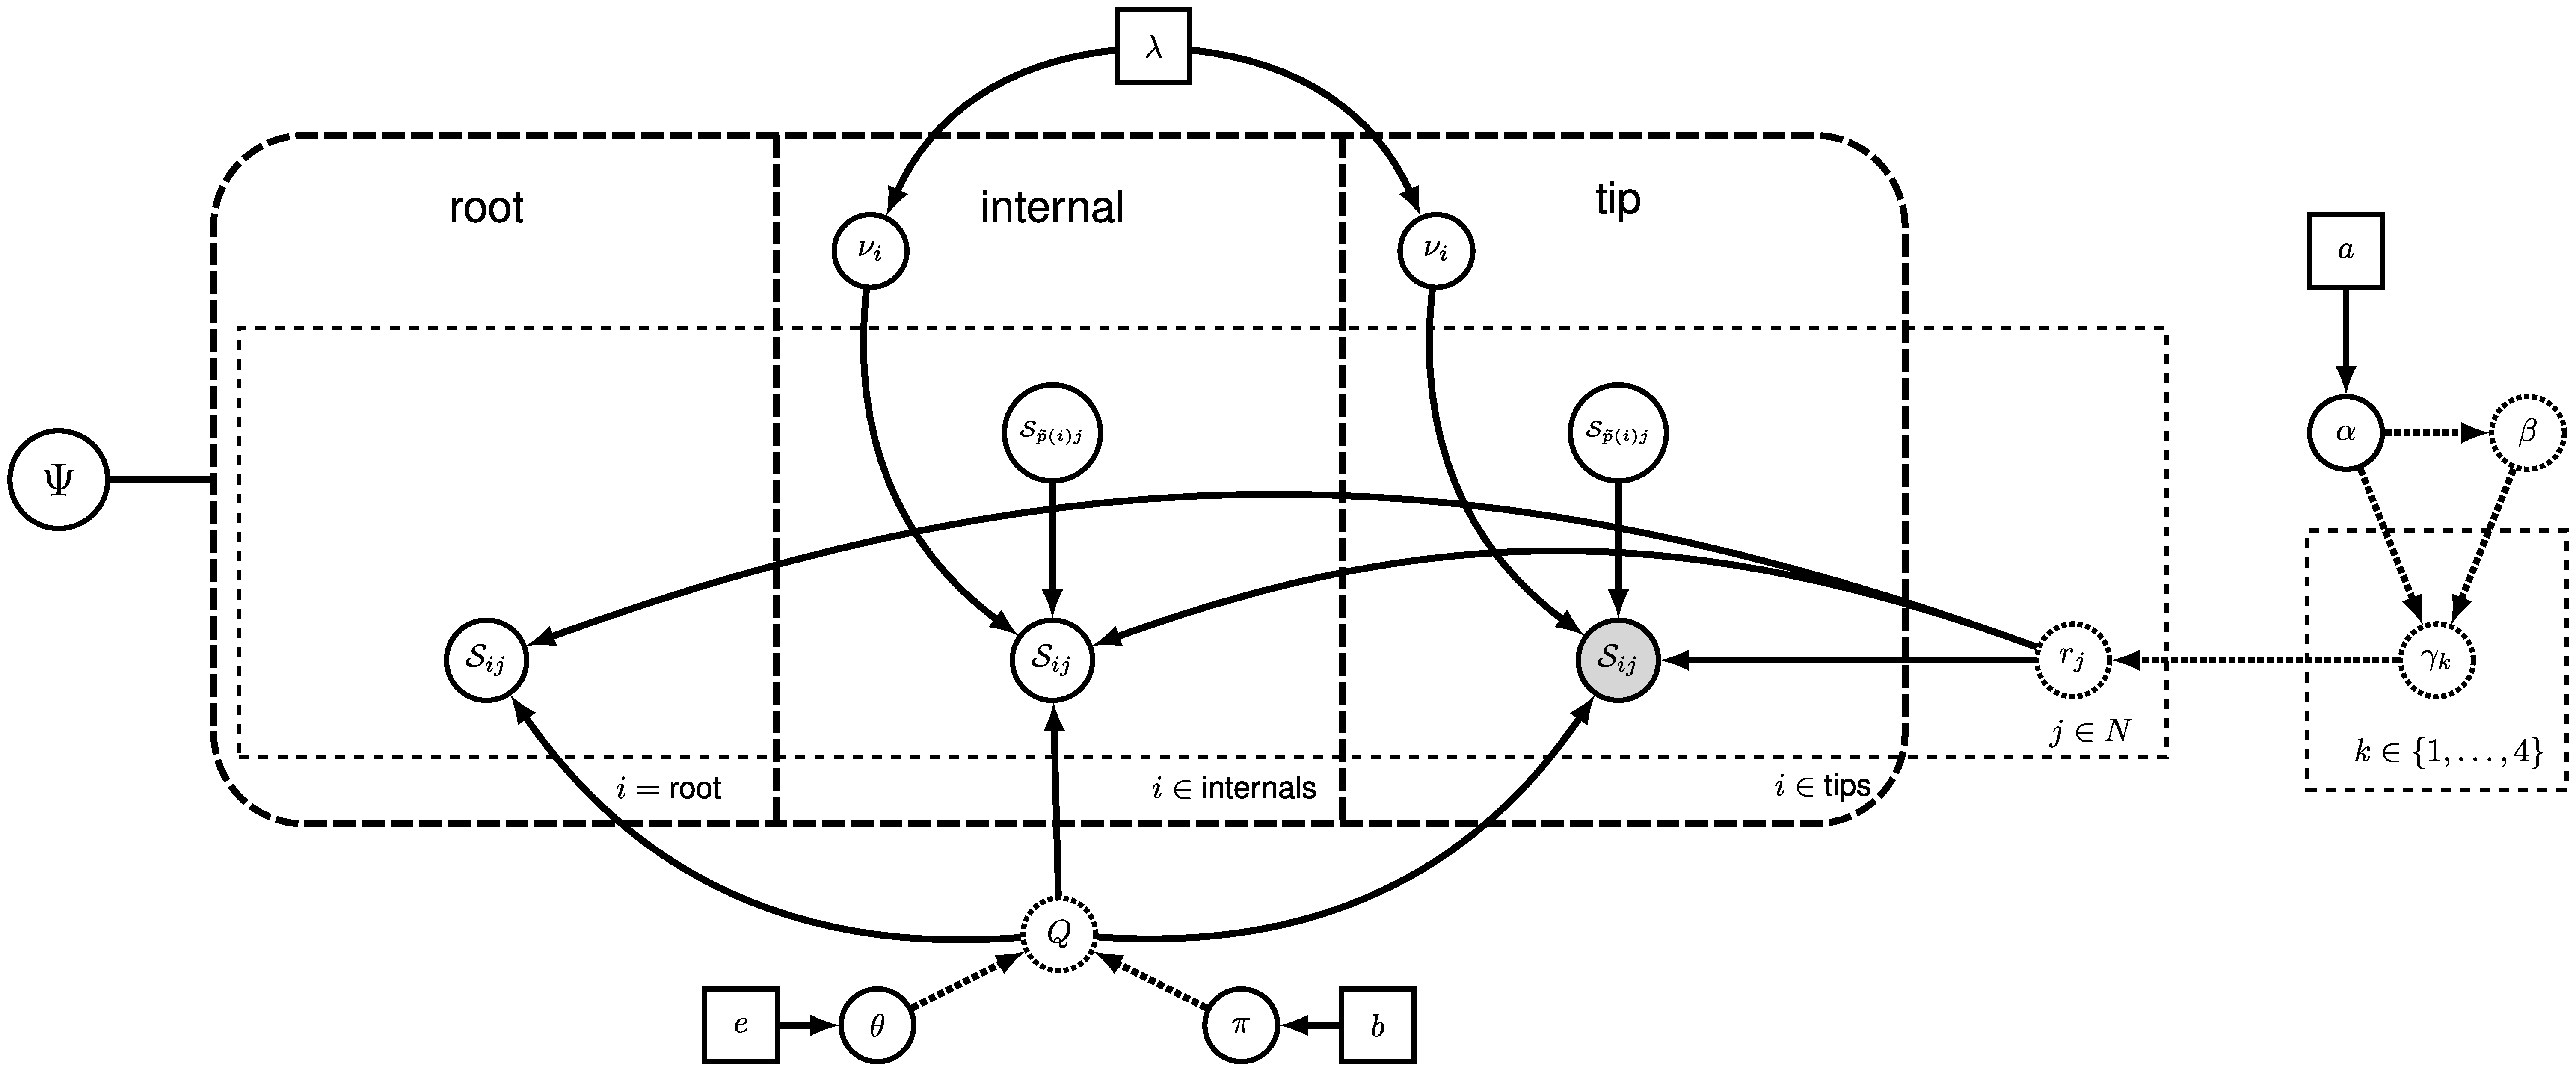
\includegraphics[width=6.8in,angle=0]{figures/gtrg_graphical_model}}
\caption{\small  The general-time reversible model \citep{tavare86} with gamma-distributed rate variation across sites \citep{yang94a}: GTR$+\Gamma$. 
The tree plate separates the nodes of the tree into different categories. For any tree there is a vector of tip nodes, a vector of internal nodes, and a root node. 
The stochastic node $\Psi$ orders the nodes in the tree plate. This representation allows for a simpler presentation of a complex model on a tree.
Each internal and tip node have a branch length applied to the branch connecting to the parent node. The branch length for node $i$ is denoted by the stochastic node $\nu_i$, and every branch-length node is conditioned on the rate parameter $\lambda$ of the exponential hyperprior.
The parameters of the GTR model include the exchangability rates $\theta$ and the equilibrium base frequencies $\pi$. 
The node $\theta$ is dependent on the constant hyperparameter $e$ which represents the vector of concentrations that control the Dirichlet prior on the stochastic node $\theta$.
Likewise, the stochastic node $\pi$ depends on the Dirichlet parameters specified in $b$.
The site rate model represented here is the discretized gamma model over four rate categories.
The stochastic node denoted $\alpha$ controls the shape of that gamma distribution.
The rate parameter $\beta$ of the gamma distribution is a deterministic node. Since we assume that the mean of the distribution on site rates is equal to $1$, then the function that determines the value of $\beta$ is $\beta = \alpha$.
The density of the gamma is discretized into 4 rate categories and the rate for each category is $\gamma_k$, for $k \in {1,\ldots,4}$. 
Then a rate value is computed for each site: $r_j$ for $j \in N$, where $N$ is the number of sites. 
}
\label{gtrgmfig}
\end{figure}

For any phylogenetic model using homologous characters, the state at the tips --- e.g., the nucleotide at a given position in the alignment --- is the observed value and clamped to the phylogenetic continuous-time Markov chain (CTMC). 
The state at any node is conditionally dependent on the sate of the parent node, thus knowing the topological ordering of nodes is important. 
Further, the state at any node is also dependent on other variables, such as the branch length, site rate, base frequencies, and relative substitution rates in a GTR$+\Gamma$ model as in Figure \ref{gtrgmfig}. 
This structure can be shown explicitly in a graphical model by fully representing the tree \citep[for examples see][]{hoehnaGM2014}.
However, even a relatively small tree of 15 tips becomes difficult to represent in this way. 
Thus, the tree plate shows this structure and can also depict the topology as a stochastic node (fig. \ref{gtrgmfig})

\bigskip
\subsection{The Rev Language}

In RevBayes models and analyses are specified using an interpreted language called \textbf{Rev}. 
The Rev language bears similarities to the compiled language in WinBUGS and the interpreted R language. 
Setting up and executing a statistical analysis in RevBayes requires the user to specify all of the parameters of their model and the type of analysis (e.g., an MCMC run). 
By using an interpreted language, RevBayes enables the practitioner to build complex, hierarchical models. 


\subsubsection*{Specifying Models}

\begin{table}[h!]
\centering
\caption{Rev language node assignment operators, clamp function, and plate/loop syntax.}\label{operatorTable}
\begin{tabular}{@{\extracolsep{\fill}}l  c r }
\hline
\multicolumn{1}{l}{\textbf{Operator}} & \multicolumn{1}{c}{ } & \multicolumn{1}{r}{\textbf{Node}}  \\ 
\hline
\cl{<-} & \hspace{10mm} &  constant node\\
\cl{\rbdn} & \hspace{10mm} &  stochastic node\\
\cl{:=} & \hspace{10mm} &  deterministic node\\
\cl{node.clamp(data)} & \hspace{10mm} &  clamped node\\
\cl{for(i in 1:N)\{...\}} & \hspace{10mm} &  plate\\
\hline
\end{tabular}
\end{table}

The nodes representing parameters of a statistical model are created using different operators in the Rev language (Table \ref{operatorTable}). 
In Figure \ref{revgmexample}, the Rev syntax for creating the model in Figure \ref{simpleGM} is provided.
Because Rev is an interpreted language, it is important to consider the order in which you specify your model. Thus, typically the first nodes that are instantiated are \textit{constant nodes}. 
Constant nodes require you to assign a fixed value to the parameter using the \cl{<-} operator. 
Stochastic nodes are initialized using the \cl{\rbdn} operator followed by the constructor function for a distribution. In the Rev language, the naming convention for distributions is \cl{dn*}, where \cl{*} is a wildcard representing the name of the distribution. Each distribution function requires hyperparameters passed in as arguments. 
This is effectively linking nodes using arrows in the graphical model.
The following specifies a stochastic node called \cl{M} which is assigned a gamma-distributed hyperprior, with shape \cl{alpha} and rate \cl{beta}:
{\tt \begin{snugshade*}
\begin{lstlisting}
alpha <- 2.0
beta <- 4.0
M ~ dnGamma(alpha, beta)
\end{lstlisting}
\end{snugshade*}}

The flexibility gained from the graphical model framework and the interpreted language allows you to easily change a model by swapping components. 
For example, if you decide that a bimodal lognormal distribution is a better representation of your uncertainty in \cl{M}, then you can simply change the distribution associated with \cl{M} (after initializing the bimodal lognormal hyperparameters):
{\tt \begin{snugshade*}
\begin{lstlisting}
mean_1 <- 0.5
mean_2 <- 2.0
sd_1 <- 1.0
sd_2 <- 1.0
weight <- 0.5
M ~ dnBimodalLnorm(mean_1, mean_2, sd_1, sd_2, weight)
\end{lstlisting}
\end{snugshade*}}

The Rev language does allows you to specify constant-node values in the distribution constructor function, therefore this also works:
{\tt \begin{snugshade*}
\begin{lstlisting}
M ~ dnBimodalLnorm(0.5, 2.0, 1.0, 1.0, 0.5)
\end{lstlisting}
\end{snugshade*}}



\begin{figure}[h!]
\centering
\fbox{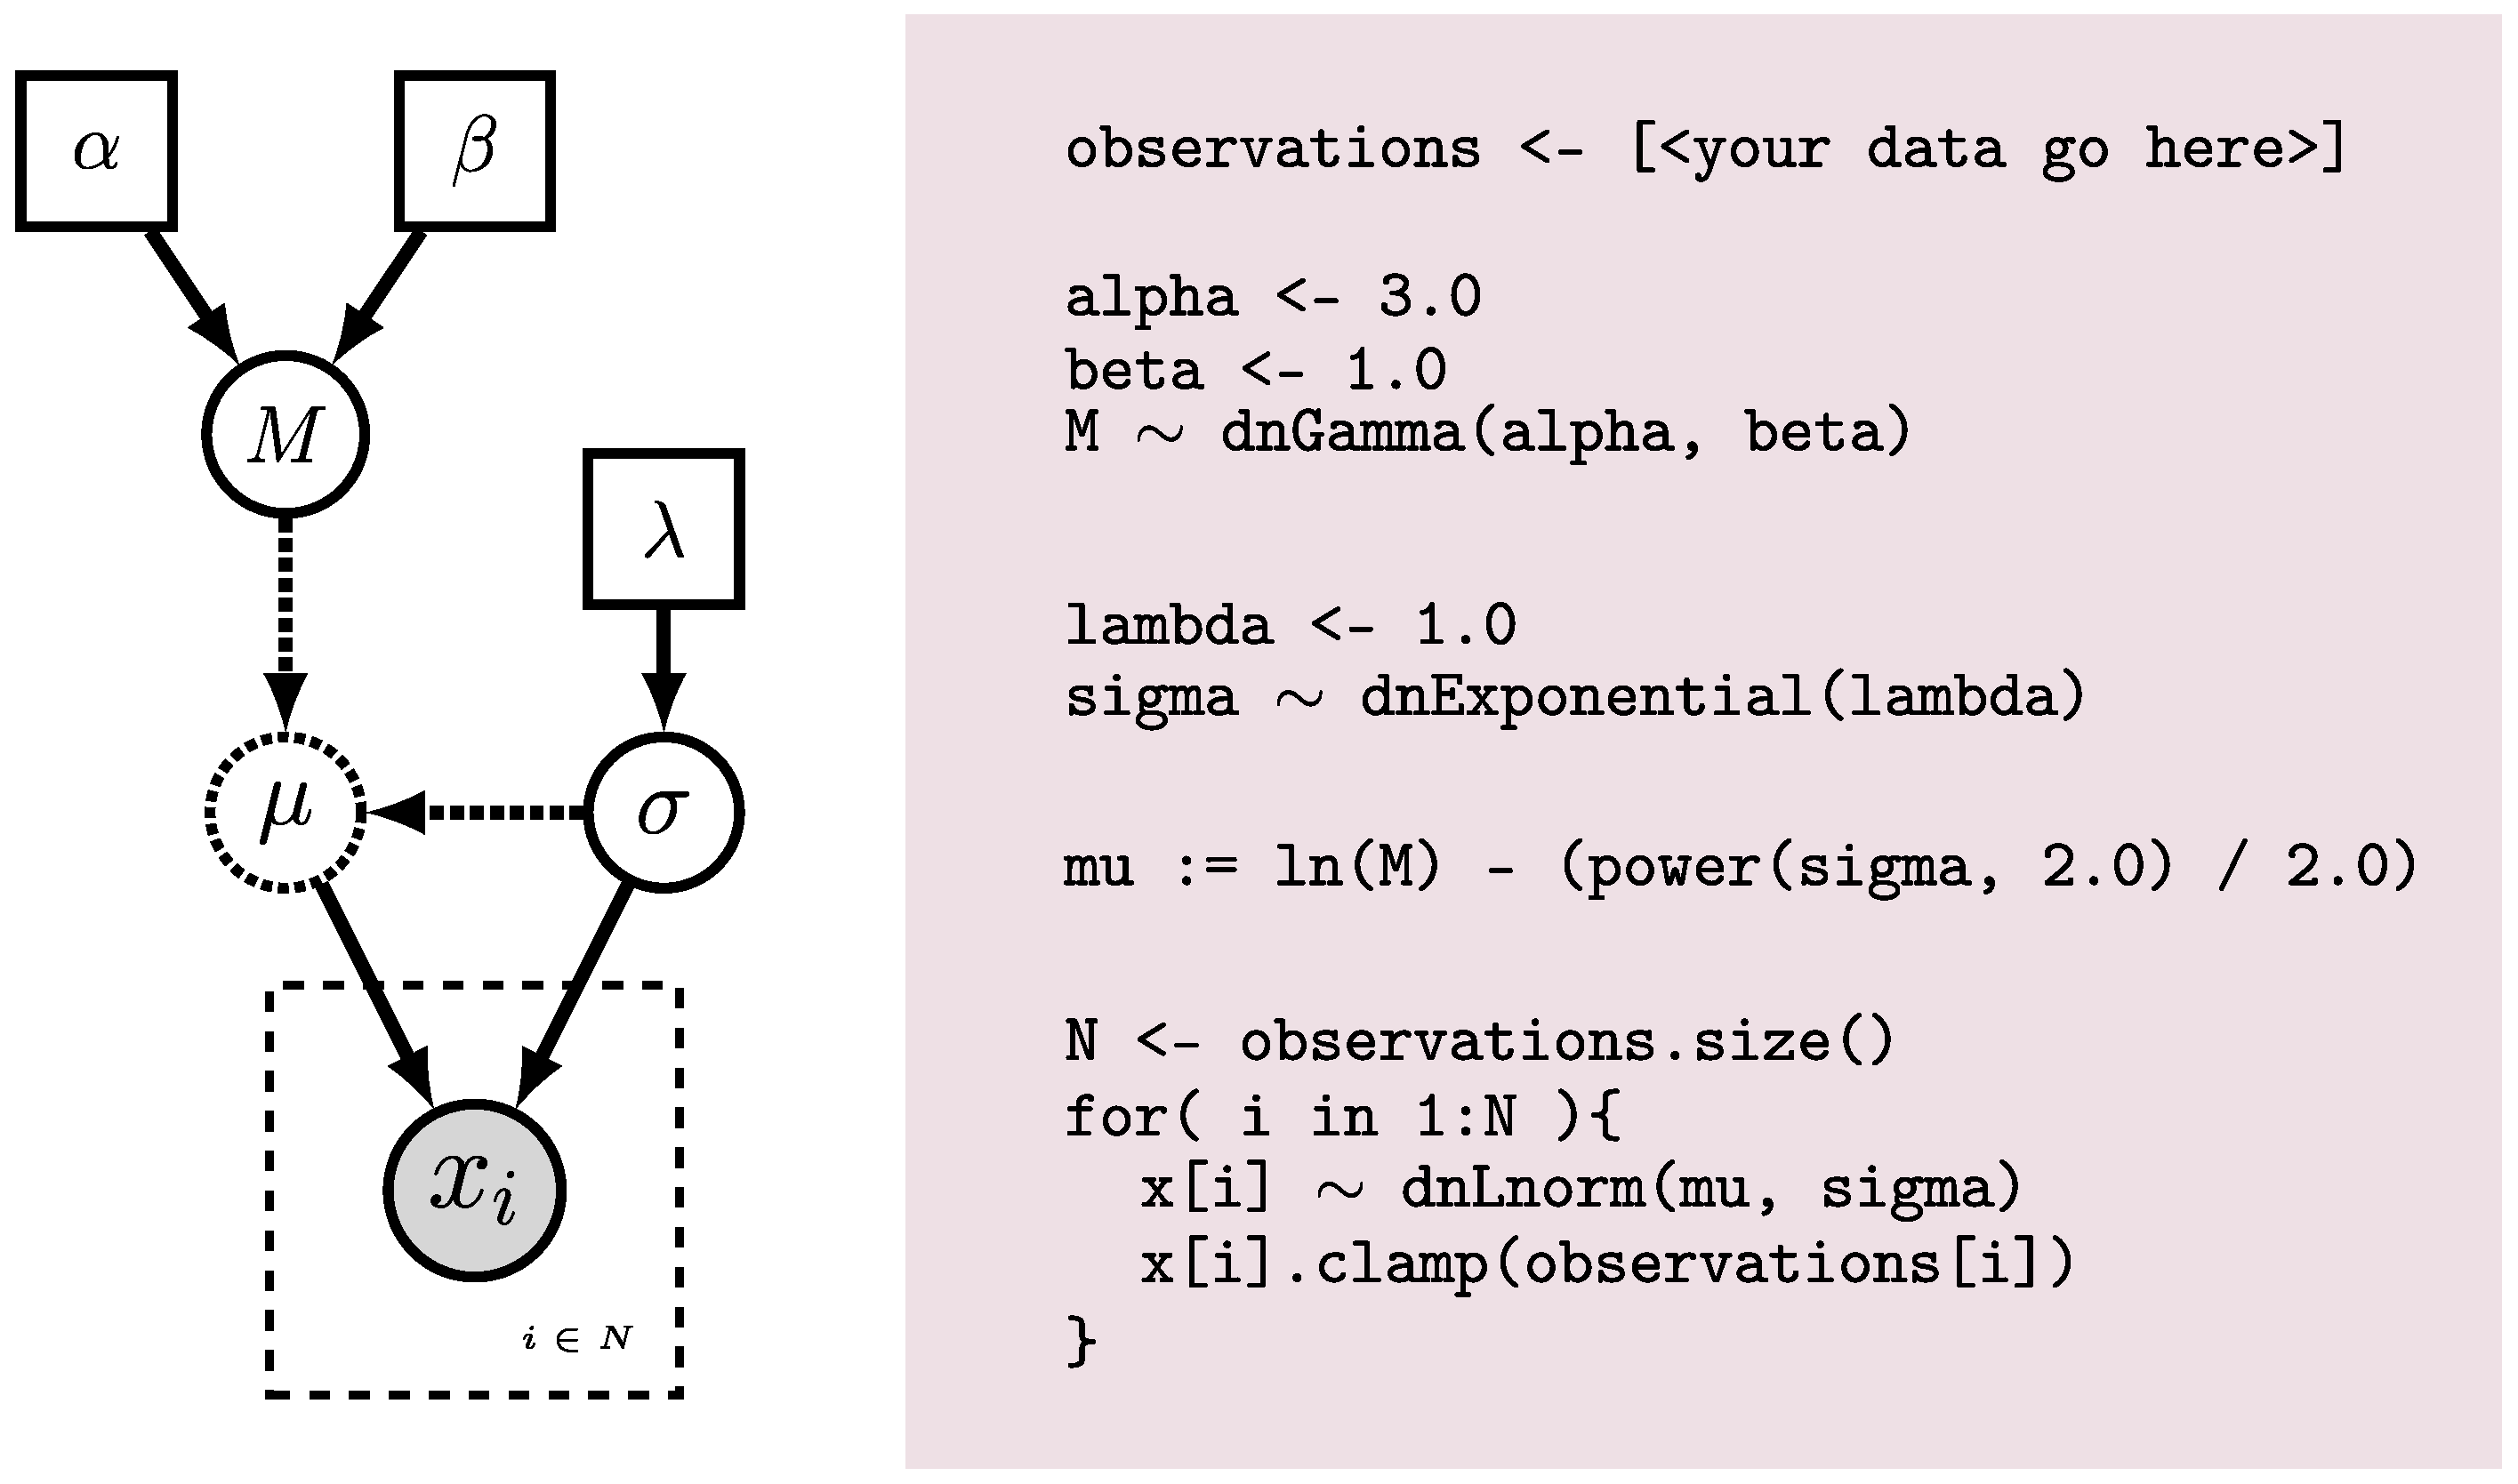
\includegraphics[width=5in,angle=0]{figures/simple_GM_rev.eps}}
\caption{\small Specifying a model in the Rev language. The graphical model of the observed parameter $x$ is shown on the left. 
In this example, $x$ is log-normally distributed with a location parameter of $\mu$ and a standard deviation of 
$\sigma$, thus $x \sim \mbox{Lognormal}(\mu, \sigma)$. The expected value of $x$ (or mean) is equal to $M$: $\mathbb{E}(x) = M$. 
In this model, $M$ and $\sigma$ are random variables and each are assigned hyperpriors. 
We assume that the mean is drawn from a gamma distribution with shape parameter $\alpha$ and rate parameter 
$\beta$: $M \sim \mbox{Gamma}(\alpha, \beta)$. The standard deviation of the lognormal distribution is assigned an 
exponential hyperprior with rate $\lambda$: $\sigma \sim \mbox{Exponential}(\lambda)$. 
Since we are conditioning our model on the \textit{expectation}, we must compute the location parameter ($\mu$) to 
calculate the probability of our model. 
Thus, $\mu$ is a deterministic node that is the result of the function$^*$ executed on $M$ and $\sigma$: $\mu = \ln(M) - \frac{\sigma^2}{2}$. 
Since we observe values of $x$, we \textit{clamp} this node.
{\scriptsize $^*$[Note that a current bug in the language related to nested functions means that \cl{mu := ln(M) - (power(sigma, 2.0) / 2.0)} does not correctly identify the parent nodes of \cl{mu}. To work around this, we need two additional deterministic nodes: \cl{lnM := ln(M)} and \cl{variance := power(sigma, 2.0)}. And \cl{mu} is changed to \cl{mu := lnM - (variance / 2.0)}.]}
}
\label{revgmexample}
\end{figure}

Deterministic nodes are variable transformations and initialized using the \cl{:=} operator followed by the function or formula for calculating the value. 
Thus, if you had an exponentially distributed stochastic node and you also wanted to monitor the square root of that variable, you can create a deterministic node:
{\tt \begin{snugshade*}
\begin{lstlisting}
p ~ dnExponential(1.0)
sq_p := sqrt(p)
\end{lstlisting}
\end{snugshade*}}

Replication over lists of variables as a plate object is specified using \cl{for} loops. 
A for-loop is an iterator statement that performs a function a given number of times. 
In RevBayes you can use this syntax to create a vector of 12 stochastic nodes, each drawn from a Poisson distribution:
{\tt \begin{snugshade*}
\begin{lstlisting}
rate <- 2.5
for( i in 1:12 ){
  p[i] ~ dnPoisson(rate)
}
\end{lstlisting}
\end{snugshade*}}

A clamped node is attached to observed data. Thus, you must first read in or input the data as a constant node, then clamp it to a stochastic node. 
In Figure \ref{revgmexample} the observations are assigned and clamped to the stochastic nodes.
If we observed 7 values for \cl{x} we would create 7 clamped nodes:
{\tt \begin{snugshade*}
\begin{lstlisting}
observations <- [0.20, 0.21, 0.03, 0.40, 0.65, 0.87, 0.22]
N <- observations.size()
for( i in 1:N ){
  x[i] ~ dnLognormal(mu, sigma)
  x[i].clamp(observations.clamp)
}
\end{lstlisting}
\end{snugshade*}}


\vspace{5mm}

{\begin{framed}
\begin{center}
Continue on to the next page to start the exercise...
\end{center}
\end{framed}}



%
%\subsection*{Analysis Functions}
%
\newpage
\FloatBarrier
\section{Exercise: Model Selection \& Partitioning using Bayes Factors}

\subsection{Introduction}
%
%
%\bigskip
%\section{Model Selection \& Partitioning using Bayes Factors}

Variation in the evolutionary process across the sites of nucleotide 
sequence alignments is well established, and is an increasingly pervasive feature of datasets 
composed of gene regions sampled from multiple loci and/or different genomes.
Inference of phylogeny from these data demands that we adequately model the underlying process heterogeneity; 
failure to do so can lead to biased estimates of phylogeny and other parameters \citep{brown07}.
To accommodate process heterogeneity within and/or between various gene(omic)
regions, we will evaluate the support for various partition schemes 
using Bayes factors to compare the marginal likelihoods of the candidate partition schemes.

Accounting for process heterogeneity involves adopting a `mixed-model' approach, \citep{ronquist03} in which the sequence alignment is first parsed into a number of partitions that are intended to capture plausible process heterogeneity within the data.
The determination of the partitioning scheme is guided by biological considerations regarding the dataset at hand.
For example, we might wish to evaluate possible variation in the evolutionary process within a single gene region ({\it e.g.}, between stem and loop regions of ribosomal sequences), or among gene regions in a concatenated alignment ({\it e.g.}, comprising multiple nuclear loci and/or gene regions sampled from different genomes).
The choice of partitioning scheme is up to the investigator and many possible partitions might be considered for a typical dataset.

Next, a substitution model is specified for each predefined process partition (using a given model-selection criterion, such as Bayes factors).
In this exercise, we assume that each partition evolved under an independent general-time reversible model with gamma-distributed rates across sites (GTR+$\Gamma$). 
Under this model the observed data are conditionally dependent on the exchangeability rates ($\theta$), stationary base frequencies ($\pi$), and the degree of gamma-distributed among-site rate variation ($\alpha$), as well as the unrooted tree topology ($\Psi$) and branch lengths ($\nu$).
We show the graphical model representation of the GTR+$\Gamma$ mode in Figure \ref{gtrgmfig}. 
When we assume different GTR+$\Gamma$ models for each partitions, this results in a composite model, in which all sites are assumed to share a common, unrooted tree topology and proportional branch lengths, but subsets of sites (`data partitions') are assumed to have independent substitution model parameters.
This composite model is referred to as a \emph{mixed model}. %\taha{need to change the graphical model above to have the same symbols as in this paragraph since this refers to the figure \ref{pipeline} and it may be harder to change that figure.}



Finally, we perform a separate MCMC simulation to approximate the joint posterior probability density of the phylogeny and other parameters.  Note that, in this approach, the mixed model is a fixed assumption of the inference ({\it i.e.}, the parameter estimates are conditioned on the specified mixed model), and the parameters for each process partition are independently estimated.

For most sequence alignments, several (possibly many) partition schemes of varying complexity are plausible {\it a priori}, which therefore requires a way to objectively identify the partition scheme that balances estimation bias and error variance associated with under- and over-parameterized mixed models, respectively.
Increasingly, mixed-model selection is based on \textit{Bayes factors} \citep[{\it e.g.},][]{suchard01}, which involves first calculating the marginal likelihood under each candidate partition scheme and then comparing the ratio of the marginal likelihoods for the set of candidate partition schemes \citep{brandley05,nylander04,mcguire07}.
The analysis pipeline that we will use in this tutorial is depicted in Figure \ref{pipeline}.
\begin{figure}[h!]
\centering
\fbox{\includegraphics[width=6.8in,angle=0]{figures/pipeline.eps}}
\caption{\small The analysis pipeline for Exercise 1. We will explore three partition schemes for the conifer dataset.
The first model (the `uniform model', $M_0$) assumes that all sites evolved under a common GTR+$\Gamma$ substitution model.
The second model (the `moderately partitioned' model, $M_1$) invokes two data partitions corresponding to the two gene regions (atpB and rbcL), and assumes each subset of sites evolved under an independent GTR+$\Gamma$ model.
The final mixed model (the `highly partitioned' model, $M_2$) invokes four data partitions---the first partition corresponds to the atpB gene region, and the remaining partitions correspond to the three codon positons of the rbcL gene region---and each data partition is assumed evolved under an independent GTR+$\Gamma$ substitution model.
Note that we assume that all sites share a common tree topology, $\Psi$, and branch-length proportions, $\nu$, for each of the candidate partition schemes.
We perform two separate sets of analyses for each mixed model---a Metropolis-coupled MCMC simulation to approximate the joint posterior probability density of the mixed-model parameters, and a `stepping-stone' MCMC simulation to approximate the marginal likelihood for each mixed model.
The resulting marginal-likelihood estimates are then evaluated using Bayes factors to assess the fit of the data to the three candidate mixed models.  
}
\label{pipeline}
\end{figure}
 
Given two models, $M_0$ and $M_1$, the Bayes factor comparison assessing the relative plausibility of each model as an explanation of the data, $BF(M_0,M_1)$, is:
$$BF(M_0,M_1) = \frac{\mbox{posterior odds}}{\mbox{prior odds}}.$$
The posterior odds is the posterior probability of $M_0$ given the data, $\mathbf X$, divided by the posterior odds of $M_1$ given the data:
$$\mbox{posterior odds} = \frac{\mathbb{P}(M_0 \mid \mathbf X)}{\mathbb{P}(M_1 \mid \mathbf X)},$$
and the prior odds is the prior probability of $M_0$ divided by the prior probability of $M_1$:
$$\mbox{prior odds} = \frac{\mathbb{P}(M_0)}{\mathbb{P}(M_1)}.$$
Thus, the Bayes factor measures the degree to which the data alter our belief regarding the support for $M_0$ relative to $M_1$ \citep{lavine99}:
\begin{align}\label{BFeq1}
BF(M_0,M_1) = \frac{\mathbb{P}(M_0 \mid \mathbf X, \theta_0)}{\mathbb{P}(M_1 \mid \mathbf X, \theta_1)} \div \frac{\mathbb{P}(M_0)}{\mathbb{P}(M_1)}. 
\end{align}
This, somewhat vague, definition does not lead to clear-cut identification of the ``best'' model. Instead, \textsl{you} must decide the degree of your belief in $M_0$ relative to $M_1$. 
Despite the absence of any strict ``rule-of-thumb'', you can refer to the scale \citep[outlined by][]{jeffreys61} for interpreting these measures (Table \ref{bftable}).
\begin{table}[h]
\centering
\caption{\small The scale for interpreting Bayes factors by Harold \citet{jeffreys61}.} 
\label{bftable}
\begin{tabular}{l c r}
\hline
\multicolumn{1}{l}{\textbf{$BF(M_0, M_1)$}} & \multicolumn{1}{r}{ } &\multicolumn{1}{r}{{Strength of evidence}} \\ 
\hline
$<1:1$ & \hspace{8mm} & Negative (supports $M_1$)\\
$1:1$ to $3:1$ & & Barely worth mentioning\\
$3:1$ to $10:1$ & & Substantial\\
$10:1$ to $30:1$ & & Strong\\
$30:1$ to $100:1$ & & Very strong\\
$>100:1$ & & Decisive\\
\hline
\multicolumn{3}{l}{{\scriptsize{For a detailed description of Bayes factors see \citet{kass95}}}} 
\end{tabular}
\end{table}


Unfortunately, direct calculation of the posterior odds to prior odds ratio is unfeasible for most phylogenetic models. However, we can further define the posterior odds ratio as:
\begin{align*}
\frac{\mathbb{P}(M_0 \mid \mathbf X)}{\mathbb{P}(M_1 \mid \mathbf X)} = \frac{\mathbb{P}(M_0)}{\mathbb{P}(M_1)} \frac{\mathbb{P}(\mathbf X \mid M_0)}{\mathbb{P}(\mathbf X \mid M_1)},
\end{align*}
where $\mathbb{P}(\mathbf X \mid M_i)$ is the \textit{marginal likelihood} of the data marginalized over all parameters for $M_i$; it is also referred to as the \textit{model evidence} or \textit{integrated likelihood}.
More explicitly, the marginal likelihood is the probability of the set of observed data ($\mathbf X$) under a given model ($M_i$), while averaging over all possible values of the parameters of the model ($\theta_i$) with respect to the prior density on $\theta_i$
\begin{align}\label{margeLike}
\mathbb{P}(\mathbf X \mid M_i) = \int \mathbb{P}(\mathbf X \mid \theta_i) \mathbb{P}(\theta_i)dt.
\end{align}
If you refer back to equation \ref{BFeq1}, you can see that, with very little algebra, the ratio of marginal likelihoods is equal to the Bayes factor:
\begin{align}\label{bfFormula}
BF(M_0,M_1) = \frac{\mathbb{P}(\mathbf X \mid M_0)}{\mathbb{P}(\mathbf X \mid M_1)} = \frac{\mathbb{P}(M_0 \mid \mathbf X, \theta_0)}{\mathbb{P}(M_1 \mid \mathbf X, \theta_1)} \div \frac{\mathbb{P}(M_0)}{\mathbb{P}(M_1)}. 
\end{align}
Therefore, we can perform a Bayes factor comparison of two models by calculating the marginal likelihood for each one. % Simple as pie, right?
Alas, exact solutions for calculating marginal likelihoods are not known for phylogenetic models (see equation \ref{margeLike}), thus we must resort to numerical integration methods to estimate or approximate these values. 
In this exercise, we will estimate the marginal likelihood for each partition scheme
using both the stepping-stone \citep{xie11} and path sampling estimators \citep{gelman1998,lartillot06, friel2008}. 

\bigskip
\subsection{Getting Started}

%This is an in-depth tutorial on model selection and data partitioning in RevBayes and this document contains a lot of information. We will \textbf{walk through} the unpartitioned model section (Section \ref{secUnif}) and the remaining sections will be available for you to try on your own. 

This tutorial assumes that you have already downloaded, compiled, and installed RevBayes. 
We also recommend that---if you are working on a Unix machine---you put the {\tt rb} binary in your path.

For the exercises outlined in this tutorial, we will use RevBayes interactively by typing commands in the command-line console.
The format of this exercise uses \colorbox{shadecolor}{\tt lavender blush shaded boxes} to delineate important steps. 
The various RevBayes commands and syntax are specified using \cl{typewriter text}. And the specific commands that you should type (or copy/paste) into RevBayes are indicated by shaded box and prompt. For example, after opening the RevBayes program, you can load your data file:

{\tt \begin{snugshade*}
\begin{lstlisting}
RevBayes > data_atpB <- readCharacterData("data/conifer_atpB.nex")[1]
\end{lstlisting}
\end{snugshade*}}

For this command, type in the command and its options:\\ \cl{data\_atpB <- readCharacterData("data/conifer\_atpB.nex")[1]}. \textbf{DO NOT} type in ``\cl{RevBayes >}'', the prompt is simply included to replicate what you see on your screen. 

Multi-line entries, particularly loops, will often be displayed in boxes without the \cl{RevBayes >} prompt so that they can be copied and pasted wholly. 
{\tt \begin{snugshade*}
\begin{lstlisting}
for( i in 1:12 ){
  x[i] ~ dnExponential(1.0)
}
\end{lstlisting}
\end{snugshade*}}


%Screen output resulting from the execution of a function or command will be in \colorbox{shadecolor}{\textcolor{outputcol}{\cl{forest green typewriter text in a shaded box}}}: 
%
%{\tt\begin{snugshade*}
%{\textcolor{outputcol}{ 
%\begin{lstlisting}
%Successfully read one character matrix from file `data/conifer\_dna.nex'
%\end{lstlisting}}}
%\end{snugshade*}}


This tutorial also includes hyperlinks: bibliographic citations are {\textcolor{citescol}{burnt orange}} and link to the full citation in the references, external URLs are {\textcolor{urlscol}{cerulean}}, and internal references to figures and equations are {\textcolor{linkscol}{purple}}.

The various exercises in this tutorial take you through the steps required to perform phylogenetic analyses of the example datasets. 
In addition, we have provided the output files for every exercise so you can verify your results. (Note that since the MCMC runs you perform will start from different random seeds, the output files resulting from your analyses \textit{will not} be identical to the ones we provide you.)

\exs{Download data and output files from: \href{https://molevol.mbl.edu/index.php/RevBayes}{https://molevol.mbl.edu/index.php/RevBayes}
%\href{http://treethinkers.org/phylogenetic-inference-using-mrbayes-v3-2/}{\small link}
}


\exs{Open the file \cl{data/conifer\_atpB.nex} in your text editor. This file contains the sequences for the atpB gene sampled from 9 species (Box 1). The elements of the \cl{DATA} block indicate the type of data, number of taxa, and length of the sequences.}


\begin{center}
Box 1: A fragment of the NEXUS file containing the atpB sequences for this exercise. \\
\end{center}
{\tt \scriptsize \begin{framed}
\begin{lstlisting}
#NEXUS 

Begin data;
	Dimensions ntax=9 nchar=1394;
	Format datatype=dna gap=-;
	Matrix
Ginkgo_biloba            TTATTGGTCCAGTACTGGATGTAGCTTTTCCCCCGGGCAATATGCCTAATATTTACAATTCTTTG...
Araucaria_araucana       -----GGTCCGGTACTGGATGTATCTTTTCCTCCAGATGAAATGCCCTATATTTACAATTCTTTG...
Cedrus_deodara           TCATTGGCCCAGTACTGGA?GTCTCTTTTCCTCCAGGTAATATGCCTAATATTTACAATTCATTG...
Cupressus_arizonica      -----------------GATGTATCTTTCCCTCCAGGTAGTATGCCTAGAATTTACAATTCTTTG...
Juniperus_communis       -----------------------------------------------------------------...
Pinus_densiflora         TCATTGGCCCAGTACTGGATGTCTCTTTTCCTCCAGGTAATATGCCTAATATTTACAATTCATTG...
Podocarpus_chinensis     TCATCGGCCCTGTACTGGATGTATCTTTTCCTCCAGATGGTATGCCTTTTATTTACAATTCTTTA...
Sciadopitys_verticillata TCATTGGTCCAGTACTAGATGTATCTTTCCCTCCAGGCAATATGCCTAGAATTTACAATTCTTTG...
Taxus_baccata            TTATCGGCCCAGTACTAGATGTCTCTTTTCCTCCAGGTAATATGCCTAAAATTTACAATTCCTTA...
	;
End;
\end{lstlisting}
\end{framed}}

\exs{Also note that ``pre-cooked'' output files are provided in the download. Throughout this tutorial, you can use those files to summarize output if you do not have time to run the full analyses yourself.}


%\exs{Open the Rev file, \taha{Rev file name}, in a text editor.  This file contains 
%all of the commands required to perform the necessary analyses to explore various
%partition schemes (unpartitioned, partitioned by gene region, and partitioned by
%gene region$+$codon position).  The details of each command are described in adjacent comments, after a \cl{\#}; {\it e.g.}, \cl{\# this is a Rev comment}. }

%Typically, we would perform these analyses by simply sourcing these files in RevBayes. For the purposes of this exercise, however, we will walk through the different steps interactively in the command line.

\bigskip
\subsection{Launch RevBayes}

Execute the RevBayes binary. If this program is in your path, then you can simply type in your Unix terminal:

\exs{\cl{\$ rb}}

When you execute the program, you will see the program information, including the current version number and functions that will provide information about the program --- \cl{contributors()} and \cl{license()}. % --- and a command reference \cl{help}. 
%Execute the \cl{help()} function by typing:
%
%{\tt \begin{snugshade*}
%\begin{lstlisting}

%RevBayes > help()
%\end{lstlisting}
%\end{snugshade*}}

%\taha{will there be help information by this time?}
%
%This displays a list of the different elements and commands available in RevBayes. The \cl{help} command also provides more detailed information about each of these items.
%
%For example, we can view the \cl{help()} information about the \cl{log()} function:
%

Currently, the help-system of RevBayes is virtually nonexistent. This will not always be the case, but is par for the course when using new/experimental software. 
The most complete help file available is for the \cl{mcmc()} function. Display the help for this function using the \cl{?} symbol:
{\tt \begin{snugshade*}
\begin{lstlisting}
RevBayes > ?mcmc
\end{lstlisting}
\end{snugshade*}}

Additionally, RevBayes will print the correct usage of a function if it is executed without any arguments:
{\tt \small \begin{snugshade*}
\begin{lstlisting}
RevBayes > mcmc()
   Error:   Argument mismatch for call to function 'mcmc'( ). Correct usage is:
   MCMC function (Model model, VectorRbPointer<Monitor> monitors,
   VectorRbPointer<Move> moves, String moveschedule = sequential|random|single)
\end{lstlisting}
\end{snugshade*}}


%allows you to save all of the screen output from your analysis to a log file. 
%The \cl{help} information for this command displays all of the available options for specifying screen logging.
%We are going to log our screen output to a file called \cl{conifer-partn-log.txt}.
%\mbcl{log start filename=conifer-partn-log.txt}
%
%Next, load the sequences into the program using the \cl{execute} command.
%\mbcl{execute conifer\_dna.nex}

%\bigskip
%\subsubsection*{Load the Sequences}% \& Specify the Outgroup}




\bigskip
\subsection{An Unpartitioned Analysis}\label{secUnif} 

{\large \textcolor{mycol}{\textsc{Black Box Analysis}}}

The first section of this exercise involves 
(1) setting up a uniform GTR+$\Gamma$ model for an alignment comprising two genes, 
(2) approximating the posterior probability of the tree topology and branch lengths (and all other parameters) using MCMC,  
(3) summarizing the MCMC output by computing the maximum a posteriori tree, and
(4) estimating the marginal likelihood of the model using stepping-stone and path sampling. 

All of the files for this analysis are provided for you and you can run these without significant effort using the \cl{source()} function in the RevBayes console:
{\tt \begin{snugshade*}
\begin{lstlisting}
RevBayes > source("RevBayes_scripts/quick_uniform.Rev")
\end{lstlisting}
\end{snugshade*}}

If everything loaded properly, then you should see the program begin running the power posterior analysis needed for estimating the marginal likelihood. If you continue to let this run, then you will see it output the states of the Markov chain once the MCMC analysis begins. (It is worth noting, however, that the file \cl{quick\_uniform.Rev} performs shorter runs with fewer generations for a faster run time.)

Ultimately, this is how you will execute most analyses in RevBayes and the full specification of the model and analyses are contained in the sourced files. 
You could easily run this entire analysis on your own data if you changed the name of the files containing the tutorial's sequences in the model specification file: \cl{RB\_tutorial\_files/uniform\_partition\_model.Rev}. 
However, it is important to understand the components of the model to be able to take advantage of the flexibility and richness of RevBayes.
Furthermore, without inspecting the Rev scripts sourced in \cl{quick\_uniform.Rev}, you may have inadvertently conducted an inappropriate analysis on your dataset, which would be a waste of your time and CPU cycles. 
The next steps will walk you through the full specification of the model and MCMC analyses. 

\bigskip
{\large \textcolor{mycol}{\textsc{Full Model Specification}}}

\textbf{\textit{Load Data}}

First load in the sequences using the \cl{readCharacterData()} function. This function returns a \textit{vector} of data matrices and, even though there is only one element in the vector, we must index that element using the \cl{[1]} notation. (You will also note that list indexing in Rev starts with \cl{1} like in the R language.)
{\tt \begin{snugshade*}
\begin{lstlisting}
RevBayes > data_atpB <- readCharacterData("data/conifer_atpB.nex")[1]
RevBayes > data_rbcL <- readCharacterData("data/conifer_rbcL.nex")[1]
\end{lstlisting}
\end{snugshade*}}
Executing these lines initializes each data matrix as their respective Rev variables. 
Since the first step in this exercise is to assume a single model for both genes, we need to combine the two datasets.
Concatenate the two data matrices using the \cl{+} operator. This returns a single data matrix with both genes.

{\tt \begin{snugshade*}
\begin{lstlisting}
RevBayes > data <- data_atpB + data_rbcL
\end{lstlisting}
\end{snugshade*}}

To report the current value of any variable, simply type the variable name and press enter. For the \cl{data} matrix, this provides information about the alignment:


{\tt \begin{snugshade*}
\begin{lstlisting}
RevBayes > data
   Origination:                   conifer_atpB.nex
   Number of taxa:                9
   Number of characters:          2659
   Number of included characters: 2659
   Datatype:                      DNA
\end{lstlisting}
\end{snugshade*}}


%\taha{can we specify an outgroup?}

%Now that RevBayes has read in our data, we can define our outgroup taxon. Unless a clock-based analysis is specified, MrBayes v3.2 infers {\em unrooted} trees, however trees are written to output files as rooted trees (unrooted trees are not phylogenies as they do not specify a temporal direction). 
%Accordingly, this command specifies how we would like our trees written to file.
%If we do not specify an outgroup, the trees will be rooted on the first species in the data matrix by default. 
%\mbcl{outgroup Ginkgo\_biloba}

Next we will specify some useful variables based on our dataset. The variable \cl{data} has \textit{member functions} that we can use to retrieve information about the dataset. 
These include the number of species (\cl{n\_species}), the tip labels (\cl{names}), and the number of internal branches (\cl{n\_branches}).
Each of these variables will be necessary for setting up different parts of our model.
{\tt \begin{snugshade*}
\begin{lstlisting}
RevBayes > n_species <- data.ntaxa()
RevBayes > names <- data.names()	
RevBayes > n_branches <- 2 * n_species - 3 
\end{lstlisting}
\end{snugshade*}}

Now we can proceed with building our GTR$+\Gamma$ model.

\textbf{\textit{The GTR Parameters}}

The first step in this exercise involves estimating the marginal likelihood of our model assuming an unpartitioned alignment. 
This corresponds to the assumption that the process that gave rise to our data was homogeneous across all sites. 
Specifically, we will assume that both genes evolved under the same GTR$+\Gamma$ model (Fig.~\ref{pipeline}). 

%\taha{describe setting up model and some background on GTR...}

%The \cl{lset} command is used to specify the details of our sequence model. 
%\mbcl{lset nst=6 rates=gamma}

%This command specifies a substitution matrix with six relative substitution rates (GTR) with gamma-distributed rate variation across sites. 
%Because models are specified this way, it is apparent that some types of DNA models are not available in MrBayes. Thus, with the \cl{nst} element of the \cl{lset} command, we can specify the JC69 or F81 models (\cl{nst=1}), the K2P or HKY models (\cl{nst=2}), or the GTR model (\cl{nst=6}).
%
%The Bayesian perspective views parameters as random variables, which requires that we specify a prior probability density that describes the precise nature of that random variation. 
%Accordingly, we need to specify priors for all of the parameters of the specified nucleotide substitution model. 
%The command for modifying priors is the \cl{prset} command. 
%
%Use the \cl{help} command to view the list of priors available for modification:
%
%\mbcl{help prset}

First, we will define and specify a prior on the exchangeability rates of the GTR model. We will use a flat Dirichlet prior distribution on these six rates. To do this, we must begin by defining a constant node that specifies the vector of concentration values of the Dirichlet prior using the \cl{v()} function:
{\tt \begin{snugshade*}
\begin{lstlisting}
RevBayes > er_prior <- v(1,1,1,1,1,1) 
\end{lstlisting}
\end{snugshade*}}


The constant node \cl{er\_prior} corresponds to the node labeled $e$ in the graphical model depicted in Figure \ref{gtrgmfig}. 
The vector function, \cl{v()}, creates a vector of six values. 
Display the current value of \cl{er\_prior} by simply typing the variable name:
{\tt \begin{snugshade*}
\begin{lstlisting}
RevBayes > er_prior
       [ 1, 1, 1, 1, 1, 1 ]
\end{lstlisting}
\end{snugshade*}}
This node defines the parameters of the Dirichlet prior distribution on the exchangeability rates. Thus, we can create a stochastic node for the exchangeability rates using the \cl{dnDirichlet()} function, which takes a vector of values as an argument and the \cl{\rbdn} operator. Together, these create a stochastic node named \cl{er} ($\theta$ in Figure \ref{gtrgmfig}): 
{\tt \begin{snugshade*}
\begin{lstlisting}
RevBayes > er ~ dnDirichlet(er_prior)
\end{lstlisting}
\end{snugshade*}}


The Dirichlet distribution assigns probability densities to grouped parameters: {\it e.g.}, those that measure proportions and must sum to 1. 
Above, we specified a 6-parameter Dirichlet prior on the relative rates of the GTR model, where the placement of each value specified represents one of the 6 relative rates: (1) $A\leftrightarrows C$, (2) $A\leftrightarrows G$, (3) $A\leftrightarrows T$, (4) $C\leftrightarrows G$, (5) $C\leftrightarrows T$, (6) $G\leftrightarrows T$. 
The input parameters of a Dirichlet distribution are called shape parameters or concentration parameters and a value is specified for each of the 6 GTR rates. 
The expectation and variance for each variable are related to the sum of the shape parameters.
The prior above is a `flat' or symmetric Dirichlet since all of the shape parameters are equal (1,1,1,1,1,1), thus we are specifying a model that allows for equal rates of change between nucleotides, such that the expected rate for each is equal to $\frac{1}{6}$ \citep{zwickl04}.
Figure \ref{dirichletFig}a shows the probability density of each rate under this model.
If we parameterized the Dirichlet distribution such that all of the parameters were equal to 100, this would also specify a prior with an expectation of equal exchangeability rates (Figure \ref{dirichletFig}b). 
However, by increasing the shape parameters of the Dirichlet distribution, \cl{er\_prior <- v(100,100,100,100,100,100)}, would heavily restrict the MCMC from sampling sets of GTR rates in which the values were not equal or very nearly equal ({\it i.e.}, this is a very {\em informative} prior). 
We can consider a different Dirichlet parameterization if we had strong prior belief that transitions and transversions occurred at different rates.
In this case, we could specify a more informative prior density: \cl{er\_prior <- v(4,8,4,4,8,4)}. 
Under this model, the expected rate for transversions would be $\frac{4}{32}$ and the expected rate for transitions would equal $\frac{8}{32}$, and there would be greater prior probability on sets of GTR rates that matched this configuration (Figure \ref{dirichletFig}c). 
An alternative informative prior would be one where we assumed that each of the 6 GTR rates had a different value conforming to a Dirichlet(2,4,6,8,10,12). 
This would lead to a different prior probability density for each rate parameter (Figure \ref{dirichletFig}d).
Without strong prior knowledge about the pattern of relative rates, however, we can better capture our statistical uncertainty with a vague prior on the GTR rates. 
Notably, all patterns of relative rates have the same probability density under \cl{er\_prior <- v(1,1,1,1,1,1)}.
\begin{figure}[h!]
\centering
\fbox{\includegraphics[width=5in,angle=-90]{figures/dirichlet_rates.eps}}
\caption{\small Four different examples of Dirichlet priors on exchangeability rates.}
\label{dirichletFig}
\end{figure}

For each stochastic node in our model, we must also specify a proposal mechanism if we wish to sample that value. 
The Dirichlet prior on our parameter \cl{er} creates a \href{http://en.wikipedia.org/wiki/Simplex}{\textit{simplex}} of values that sum to 1. 
In RevBayes, there are many different proposal mechanisms -- called \textit{moves} -- and each move operates on a specific data type (called RevType). 
Check the RevType of the variable \cl{er} using the \cl{structure()} function:
{\tt \small \begin{snugshade*}
\begin{lstlisting}
RevBayes > structure(er)

  _variable     = er <0x7ffed8449370>
  _RevType      = Simplex
  _RevTypeSpec  = [ Simplex, RealPos[], ModelContainer, Container, RevObject ]
  _value        = [ 0.00308506, 0.491487, 0.186317, 0.0275106, 0.1982...
  _size         = 6
  _dagNode      = er <0x7ffed8448bb0>
  _dagType      = Stochastic DAG node
  _refCount     = 1
  _distribution = <0x7ffed8448cf0>
  _touched      = TRUE
  _clamped      = FALSE
  _lnProb       = -inf
  _storedLnProb = 6.95325e-310
  _parents      = [ er_prior <0x7ffed8449250> ]
  _children     = [  ]
\end{lstlisting}
\end{snugshade*}}

The \cl{structure()} function -- which has an accepted abbreviation of \cl{str()} -- is verbose and provides a lot of information that may at first appear confusing. 
In particular, this function provides the \href{http://en.wikipedia.org/wiki/Memory_address}{\textit{memory addresses}} of the node, its parent node(s), and the distribution. 
These strings indicate the location of the variable in computer memory. 
Thus, if you view the structure of your \cl{er} node, these sequences of numbers will be different from the ones in the box above. 
Much of this information is helpful primarily for troubleshooting and debugging purposes, however, the components that you may want to look at are: \cl{RevType}, \cl{value}, \cl{dagType}, \cl{clamped}, \cl{lnProb}, and the names of the \cl{variable}, \cl{parents}, and \cl{children}.

We must create a vector containing all of the moves for each of our stochastic nodes. 
This vector will be passed in to the function constructing our MCMC or power posterior runs.
All moves in the Rev language are called \cl{mv*}, where \cl{*} is a wild card for the move name. 
Initialize the first element of our vector of moves by setting the proposal on the exchangeability rates:

{\tt\small \begin{snugshade*}
\begin{lstlisting}
RevBayes > moves[1] <- mvSimplexElementScale(er, alpha=10, tune=true, weight=3) 
\end{lstlisting}
\end{snugshade*}}


The various proposal mechanisms available in RevBayes each require specific input arguments. 
The \cl{mvSimplexElementScale} move can only operate on a simplex and the first argument is the stochastic node that you wish to update. 
The variable node is followed by three more arguments: (1) \cl{alpha} is the \textit{tuning parameter} of the move and controls the size of the proposal; (2) by setting \cl{tune=true} we are telling the program to adjust the tuning parameter if the acceptance rate of the proposal is too high or too low -- the target for this move is an acceptance rate of 0.44; (3) the \cl{weight} specifies how frequently this move is performed at each step in the Markov chain. 

It is important to note that by default, a single generation in RevBayes updates all stochastic nodes in proportion to the \cl{weight} argument specified. 
This approach is different from many phylogenetic MCMC programs -- such as MrBayes -- which only perform one move per MCMC iteration. 
Instead, for each generation in RevBayes, a \textit{move list} is carried out in random order. 
By setting \cl{weight=3} above, we are ensuring that the new values are proposed for \cl{er} three times per iteration. 
Thus, if you set \cl{weight=0.5} the move will only have a 50\% chance of occurring at each generation. 
Essentially, the \cl{weight} argument for each move indicates the number of times it will be performed.
If you keep all of the move weights set to the values specified in this tutorial for the uniform model, you will have set 20 different moves and the MCMC simulator will execute 38 moves per generation.
This is a practical approach for MCMC analysis using complex models and is used by several other programs (\href{http://megasun.bch.umontreal.ca/People/lartillot/www/index.htm}{Phylobayes}, \href{http://hydrodictyon.eeb.uconn.edu/projects/phycas/index.php/Phycas_Home}{Phycas}, \href{http://www.bali-phy.org/}{Bali-Phy}).
However, because RevBayes is updating many parameters each generation, it is not straightforward to compare run-times with a program like MrBayes that only performs approximately one update per generation. 
Furthermore, using this approach to MCMC simulation, you can sufficiently sample the chain in fewer generations while sampling more frequently than you would in programs that only perform one update per step.

We can use the same type of distribution as a prior on the 4 stationary frequencies ($\pi_A, \pi_C, \pi_G, \pi_T$) since these parameters also represent proportions. 
Specify a flat Dirichlet prior density on the base frequencies:
{\tt \begin{snugshade*}
\begin{lstlisting}
RevBayes > sf_prior <- v(1,1,1,1) 
RevBayes > sf ~ dnDirichlet(sf_prior)
\end{lstlisting}
\end{snugshade*}}

The node \cl{sf} represents the $\pi$ node in Figure \ref{gtrgmfig}.
Now add the simplex scale move on the stationary frequencies to the moves vector:
{\tt \small \begin{snugshade*}
\begin{lstlisting}
RevBayes > moves[2] <- mvSimplexElementScale(sf, alpha=10, tune=true, weight=2)  
\end{lstlisting}
\end{snugshade*}}

We can finish setting up this part of the model by creating a deterministic node for the GTR rate matrix \cl{Q}. 
The \cl{gtr()} function takes a set of exchangeability rates and a set of base frequencies to compute the rate matrix used when calculating the likelihood of our model.
{\tt \begin{snugshade*}
\begin{lstlisting}
RevBayes > Q := gtr(er,sf)
\end{lstlisting}
\end{snugshade*}}


\textbf{\textit{Gamma-Distributed Site Rates}}


We will also assume that the substitution rates vary among sites according to a gamma distribution, which has two parameters: the shape parameter, $\alpha$, and the rate parameter, $\beta$. 
In order that we can interpret the branch lengths as the expected number of substitutions per site, this model assumes that the mean site rate is equal to 1.
%Consequently, we wish to specify a gamma distribution with a mean of 1.
The mean of the gamma is equal to $\alpha/\beta$, so a mean-one gamma is specified by setting the two parameters to be equal, $\alpha=\beta$.
Therefore, we need only consider the single shape parameter, $\alpha$ \citep{yang94a}. 
The degree of among-site substitution rate variation (ASRV) is inversely proportional to the value of the shape parameter---as the value of $\alpha$-shape parameter increases, the gamma distribution increasingly resembles a normal distribution with decreasing variance, which corresponds to decreasing levels of ASRV (Figure \ref{asrhGammaFig}).
If $\alpha = 1$, then the gamma distribution collapses to an exponential distribution with a rate parameter equal to $\beta$.
By contrast, when the value of the $\alpha$-shape parameter is $< 1$, the gamma distribution assumes a concave distribution that places most of the prior density on low rates but allows some prior mass on sites with very high rates, which corresponds to high levels of ASRV (Figure \ref{asrhGammaFig}).

\begin{figure}[h]
\centering
\fbox{\includegraphics[width=2.5in,angle=-90]{figures/asrh_gamma.eps}}
\caption{\small The probability density of mean-one gamma-distributed rates under different shape parameters.}
\label{asrhGammaFig}
\end{figure}


Alternatively, we might not have good prior knowledge about the variance in site rates, thus we can place an uninformative, or diffuse prior on the shape parameter.
For this analysis, we will use an exponential distribution with a rate parameter, \cl{shape\_prior}, equal to \cl{0.05}.
Under an exponential prior, we are placing non-zero probability on values of $\alpha$ ranging from 0 to $\infty$. 
The rate parameter, often denoted $\lambda$, of an exponential distribution controls both the mean and variance of this prior such that the expected (or mean) value of $\alpha$ is:
$\mathbb{E}[\alpha] = \frac{1}{\lambda}.$
Thus, if we set $\lambda=0.05$, then $\mathbb{E}[\alpha] = 20$.

Create a constant node called \cl{shape\_prior} for the rate parameter of the exponential prior on the gamma-shape parameter
{\tt\begin{snugshade*}
\begin{lstlisting}
RevBayes > shape_prior <- 0.05                                                                             
\end{lstlisting}
\end{snugshade*}}

Then create a stochastic node called \cl{shape} to represent the $\alpha$ node in Figure \ref{gtrgmfig}, with an exponential density as a prior:
{\tt\begin{snugshade*}
\begin{lstlisting}
RevBayes > shape ~ dnExponential(shape_prior)

\end{lstlisting}
\end{snugshade*}}

The way the ASRV model is implemented involves discretizing the mean-one gamma distribution into a set number of rate categories. Thus, we can analytically marginalize over the uncertainty in the rate at each site. To do this, we need a deterministic node that is a vector of rates calculated from the gamma distribution and the number of rate categories. The \cl{discretizeGamma()} function returns this deterministic node and takes three arguments: the shape and rate of the gamma distribution and the number of categories. Since we want to discretize a mean-one gamma distribution, we can pass in \cl{shape} for both the shape and rate.

Initialize the \cl{gamma\_rates} deterministic node vector using the  \cl{discretizeGamma()} function with \cl{4} bins:
{\tt \begin{snugshade*}
\begin{lstlisting}
RevBayes > gamma_rates := discretizeGamma( shape, shape, 4 )
\end{lstlisting}
\end{snugshade*}}



The random variable that controls the rate variation is the stochastic node \cl{shape}. This variable is a single, real positive value (\cl{RevType = RealPos}). 
We will apply a simple scale move to this parameter.
The scale move's tuning parameter is called \cl{lambda} and this value dictates the size of the proposal.
{\tt \begin{snugshade*}
\begin{lstlisting}
moves[3] <- mvScale(shape, lambda=1.0, tune=true, weight=2.0)\end{lstlisting}
\end{snugshade*}}


\textbf{\textit{Tree Topology and Branch Lengths}}

The tree topology and branch lengths are also stochastic nodes in our model. 
In Figure \ref{gtrgmfig}, the tree topology is denoted $\Psi$ and the length of the branch leading to node $i$ is $\nu_i$.

We will assume that all possible labeled, unrooted tree topologies have equal probability. This is the \cl{dnUniformTopology()} distribution in RevBayes. Specify the \cl{topology} stochastic node by passing in the number of species \cl{n\_species} and tip labels \cl{names} to the \cl{dnUniformTopology()} distribution:
{\tt \begin{snugshade*}
\begin{lstlisting}
RevBayes > topology ~ dnUniformTopology(n_species, names)
\end{lstlisting}
\end{snugshade*}}

For some types of stochastic nodes there are several available moves. 
Often the different moves explore parameter space in a different way and nothing prevents one from using multiple different moves to improve mixing. 
For the unrooted tree topology, we can use both a nearest-neighbor interchange move (\cl{mvNNI}) and a subtree-prune and regrafting move (\cl{mvSPR}). These moves do not have tuning parameters associated with them, thus you only need to pass in the \cl{topology} node and \cl{weight} 
{\tt \begin{snugshade*}
\begin{lstlisting}
RevBayes > moves[4] <- mvNNI(topology, weight=10.0)
RevBayes > moves[5] <- mvSPR(topology, weight=5.0)
\end{lstlisting}
\end{snugshade*}}


Next we have to create a stochastic node for each of the $2N-3$ branches in our tree (where $N=$ \cl{n\_species}). 
We can do this using a \cl{for} loop --- this is a plate in our graphical model. In this loop, we can create each branch-length node and assign each move. Copy this entire block of Rev code into the console:
{\tt \small \begin{snugshade*}
\begin{lstlisting}
mi <- 5
for (i in 1:n_branches) {
   br_lens[i] ~ dnExponential(10.0)
   moves[mi++] <- mvScale(br_lens[i],lambda=1,tune=true,weight=1) 
}
\end{lstlisting}
\end{snugshade*}}

It is convenient to monitor a deterministic variable of the branch lengths. In MrBayes, \textit{tree length} was reported to the log file instead of the length of each branch. The tree length is the sum of all branch lengths and this can be computed using the \cl{sum()} function which calculates the sum of any vector of values.
{\tt \begin{snugshade*}
\begin{lstlisting}
RevBayes > tree_length := sum(br_lens)
\end{lstlisting}
\end{snugshade*}}

Finally, we can create a branch-length phylogeny by combining the tree topology and branch lengths using the \cl{treeAssembly()} function, which applies the value of the $i^{th}$ member of the \cl{br\_lens} vector to the branch leading to the $i^{th}$ node in \cl{topology}. Thus, the \cl{phylogeny} variable is a deterministic node: 

{\tt \begin{snugshade*}
\begin{lstlisting}
RevBayes > phylogeny := treeAssembly(topology, br_lens)
\end{lstlisting}
\end{snugshade*}}



\textbf{\textit{Putting it All Together}}

Now that we have initialized virtually all of our model parameters and we can link all of the parts in the stochastic node that will be clamped by the data. 
The sequence substitution model is a distribution called the \textit{phylogenetic continuous-time Markov chain} and we use the \cl{dnPhyloCTMC} constructor function to create this node.
This distribution requires several input arguments: (1) the \cl{tree} with branch lengths, (2) the instantaneous rate matrix \cl{Q}, the node characterizing the rate variation across sites (though \cl{siteRates} can be omitted if you do not assume rate variation across sites), (3) \cl{nSites} is the number of sites in the alignment, and (4) the \cl{type} of character data.
{\tt \begin{snugshade*}
\begin{lstlisting}
RevBayes > phyloSeq ~ dnPhyloCTMC(tree=phylogeny, Q=Q, siteRates=gamma_rates, nSites=data.nchar(1), type="DNA")
\end{lstlisting}
\end{snugshade*}}


Once the character evolution model has been created, we can attach our sequence data to the tip nodes in the tree.
{\tt \begin{snugshade*}
\begin{lstlisting}
RevBayes > phyloSeq.clamp(data)
\end{lstlisting}
\end{snugshade*}}
When this function is called, RevBayes sets each of the stochastic nodes representing the tip nodes of the tree to the sequence corresponding to that species in the alignment. 
This essentially tells the program that this is where the DAG ends and the states of the tip nodes are fixed. 

Now we can wrap up the whole model to conveniently access the DAG. To do this, we only need to give the \cl{model()} function a single node. With this node, the \cl{model()} function can find all of the other nodes by following the arrows in the graphical model:
{\tt \begin{snugshade*}
\begin{lstlisting}
RevBayes > mymodel <- model(sf)
\end{lstlisting}
\end{snugshade*}}

Now we have specified a simple, single-partition analysis---each parameter of the model will be estimated from every site in our alignment.
If we inspect the contents of \cl{mymodel} we can review all of the nodes in the DAG:
{\tt \begin{snugshade*}
\begin{lstlisting}
RevBayes > mymodel
\end{lstlisting}
\end{snugshade*}}

\bigskip
{\large \textcolor{mycol}{\textsc{Perform MCMC Analysis Under the Uniform Model}}}

This section will cover setting up the MCMC sampler and summarizing the posterior distribution of trees. 

\textbf{\textit{Specify Monitors}}

For our MCMC analysis we need to set up a vector of \textit{monitors} to save the states of our Markov chain. 
The monitor functions are all called \cl{mn*}, where \cl{*} is the wildcard representing the monitor type.
First, we will initialize the model monitor using the \cl{mnModel} function. This creates a new monitor variable that will output the states for all model parameters when passed into a MCMC function. 
{\tt \begin{snugshade*}
\begin{lstlisting}
RevBayes > monitors[1] <- mnModel(filename="output/conifer_uniform.log", printgen=100)
\end{lstlisting}
\end{snugshade*}}

The \cl{mnFile} monitor will record the states for only the parameters passed in as arguments. We use this monitor to specify the output for our sampled trees and branch lengths.

{\tt \begin{snugshade*}
\begin{lstlisting}
RevBayes > monitors[2] <- mnFile(filename="output/conifer_uniform.trees",printgen=100, phylogeny)
\end{lstlisting}
\end{snugshade*}}


Finally, create a screen monitor that will report the states of specified variables to the screen with \cl{mnScreen}:
{\tt \begin{snugshade*}
\begin{lstlisting}
RevBayes > monitors[3] <- mnScreen(printgen=10, separator = " | ", tree_length)
\end{lstlisting}
\end{snugshade*}}

\textbf{\textit{Initialize and Run MCMC}}

With a fully specified model, a set of monitors, and a set of moves, we can now set up the MCMC algorithm that will sample parameter values in proportion to their posterior probability. The \cl{mcmc()} function will create our MCMC object:
{\tt \begin{snugshade*}
\begin{lstlisting}
RevBayes > mymcmc <- mcmc(mymodel, monitors, moves)
\end{lstlisting}
\end{snugshade*}}


We can run the \cl{.burnin()} member function if we wish to pre-run the chain and discard the initial states. 
{\tt \begin{snugshade*}
\begin{lstlisting}
RevBayes > mymcmc.burnin(generations=10000,tuningInterval=1000)
\end{lstlisting}
\end{snugshade*}}


Now, run the MCMC:
{\tt \begin{snugshade*}
\begin{lstlisting}
RevBayes > mymcmc.run(generations=30000)
\end{lstlisting}
\end{snugshade*}}

When the analysis is complete, you will have the monitor files in your output directory.


\textbf{\textit{Summarize the MCMC Output}}

Methods for visualizing the marginal densities of parameter values are not currently available in RevBayes. Thus, it is important to use programs like Tracer \citep{rambaut09} to evaluate mixing and non-convergence. (RevBayes does, however, have a tool for convergence assessment called \cl{beca}.)

RevBayes can also summarize the tree samples by reading in the tree-trace file:
{\tt \begin{snugshade*}
\begin{lstlisting}
RevBayes > treetrace <- readTreeTrace("output/conifer_uniform.trees")
RevBayes > treetrace.summarize()
\end{lstlisting}
\end{snugshade*}}


The \cl{mapTree()} function will summarize the tree samples and write the maximum a posteriori tree to file:
{\tt \begin{snugshade*}
\begin{lstlisting}
RevBayes > mapTree(treetrace,"output/conifer_uniform_map.tre")
\end{lstlisting}
\end{snugshade*}}

%If you calculated the Bayes factors to determine the relative support for the uniform model and found that there was strong evidence supporting this model over others (hint: this is not true if you proceed with this tutorial and evaluate the other models), then you will want to select the uniform model for your MCMC analysis and estimate the tree.


\bigskip
{\large \textcolor{mycol}{\textsc{Estimating the Marginal Likelihood}}}

Typically, model comparison is performed prior to running the full MCMC analysis under a model. 
If you calculated the Bayes factors to determine the relative support for the uniform model and found that there was strong evidence supporting this model over others (hint: this is not true if you proceed with this tutorial), then it would be worth your time to proceed with the MCMC steps outlined above. 
The following steps will describe using stepping-stone and path sampling methods on a set of power posteriors to estimate marginal likelihoods under the uniform model. 

With a fully specified model, we can set up the \cl{powerPosterior()} analysis to create a file of `powers' and likelihoods from which we can estimate the marginal likelihood using stepping-stone or path sampling. 
This method computes a vector of powers from a beta distribution, then executes an MCMC run for each power step while raising the likelihood to that power. In this implementation, the vector of powers starts with 1, sampling the likelihood close to the posterior and incrementally sampling closer and closer to the prior as the power decreases. 



%\textbf{\textit{Clear Workspace and Load the Data and Model}}

Just to be safe, it is better to clear the workspace and re-load the data and model:
{\tt \begin{snugshade*}
\begin{lstlisting}
RevBayes > clear()
RevBayes > source("RevBayes_scripts/uniform_partition_model.Rev")
\end{lstlisting}
\end{snugshade*}}


First, we create the variable containing the power posterior. This requires us to provide a model and vector of moves, as well as an output file name. The \cl{cats} argument sets the number of power steps.
{\tt \begin{snugshade*}
\begin{lstlisting}
RevBayes > pow_p <- powerPosterior(mymodel, moves, "pow_p_uniform.out", cats=50) 
\end{lstlisting}
\end{snugshade*}}

We can start the power posterior by first burning in the chain and and discarding the first 10000 states.  
{\tt \begin{snugshade*}
\begin{lstlisting}
RevBayes > pow_p.burnin(generations=10000,tuningInterval=1000)
\end{lstlisting}
\end{snugshade*}}

Now execute the run with the \cl{.run()} function:
{\tt \begin{snugshade*}
\begin{lstlisting}
RevBayes > pow_p.run(generations=1000)  
\end{lstlisting}
\end{snugshade*}}

Once the power posteriors have been saved to file, create a stepping stone sampler. This function can read any file of power posteriors and compute the marginal likelihood using stepping-stone sampling. 
{\tt \small \begin{snugshade*}
\begin{lstlisting}
RevBayes > ss <- steppingStoneSampler(file="pow_p_uniform.out", powerColumnName="power", likelihoodColumnName="likelihood")
\end{lstlisting}
\end{snugshade*}}

Compute the marginal likelihood under stepping-stone sampling using the member function \cl{marginal()} of the \cl{ss} variable and record the value in Table \ref{ssTable}.
{\tt \begin{snugshade*}
\begin{lstlisting}
RevBayes > ss.marginal() 
\end{lstlisting}
\end{snugshade*}}

Path sampling is an alternative to stepping-stone sampling and also takes the same power posteriors as input. 
{\tt \small \begin{snugshade*}
\begin{lstlisting}
RevBayes > ps <- pathSampler(file="pow_p_uniform.out", powerColumnName="power", likelihoodColumnName="likelihood")
\end{lstlisting}
\end{snugshade*}}

Compute the marginal likelihood under stepping-stone sampling using the member function \cl{marginal()} of the \cl{ps} variable and record the value in Table \ref{ssTable}.
{\tt \begin{snugshade*}
\begin{lstlisting}
RevBayes > ps.marginal() 
\end{lstlisting}
\end{snugshade*}}


%%%%%%%%

\vspace{5mm}

{\begin{framed}
\begin{center}
Stop here or continue on to evaluate partitioned models...
\end{center}
\end{framed}}



\bigskip
\subsection{Partitioning by Gene Region}\label{secByGene}

The uniform model used in the previous section assumes that all sites in the alignment evolved under the same process described by a shared tree, branch length proportions, and parameters of the GTR+$\Gamma$ substitution model.
However, our alignment contains two distinct gene regions---atpB and rbcL---so we may wish to explore the possibility that the substitution process differs between these two gene regions.
This requires that we first specify the data partitions corresponding to these two genes, then define an independent substitution model for each data partition. 

\textbf{\textit{Clear Workspace and Reload Data}}

{\tt \begin{snugshade*}
\begin{lstlisting}
RevBayes > clear()
\end{lstlisting}
\end{snugshade*}}

Since we wish to avoid individually specifying each parameter of the GTR+$\Gamma$ model for each of our data partitions, we can \textit{loop} over our datasets and create vectors of nodes.
To do this, we begin by creating a vector of data file names:
{\tt \begin{snugshade*}
\begin{lstlisting}
RevBayes > filenames <- v("data/conifer_atpB.nex", "data/conifer_rbcL.nex")
\end{lstlisting}
\end{snugshade*}}

Set a variable for the number of partitions:
{\tt \begin{snugshade*}
\begin{lstlisting}
RevBayes > n_parts <- filenames.size()
\end{lstlisting}
\end{snugshade*}}

And create a vector of data matrices called \cl{data}:
{\tt \begin{snugshade*}
\begin{lstlisting}
for (i in 1:n_parts){
   data[i] <- readCharacterData(filenames[i])[1]
}
\end{lstlisting}
\end{snugshade*}}

Next, we can initialize some important variables. This does require, however, that both of our alignments have the same number of species and matching tip names.
{\tt \begin{snugshade*}
\begin{lstlisting}
RevBayes > n_species <- data[1].ntaxa()
RevBayes > names <- data[1].names()
RevBayes > n_branches <- 2 * n_species - 3
\end{lstlisting}
\end{snugshade*}}


\textbf{\textit{Specify the Parameters by Looping Over Partitions}}

We can avoid creating unique names for every node in our model if we use a \cl{for} loop to iterate over our partitions. Thus, we will only have to type in our entire GTR+$\Gamma$ model parameters once. 
This will produce a vector for each of the unlinked parameters --- e.g., there will be a vector of \cl{shape} nodes where the stochastic node for the first partition (atpB) will be \cl{shape[1]} and the stochastic node for the second partition (rbcL) will be called \cl{shape[2]}.
{\tt \small \begin{snugshade*}
\begin{lstlisting}
mi <- 0 # an iterator for the move vector
for (i in 1:n_parts){
  ## index i=1 : atpB gene ##
  ## index i=2 : rbcL gene ##
  
  # Exchangeability rates #
  er_prior[i] <- v(1,1,1,1,1,1)
  er[i] ~ dnDirichlet(er_prior[i])
  moves[mi++] <- mvSimplexElementScale(er[i], alpha=10, tune=true, weight=3) 

  # Stationary base frequencies #
  sf_prior[i] <- v(1,1,1,1)
  sf[i] ~ dnDirichlet(sf_prior[i])
  moves[mi++] <- mvSimplexElementScale(sf[i], alpha=10, tune=true, weight=2) 

  # Instantaneous rate matrix (deterministic) #
  Q[i] := gtr(er[i],sf[i]) 

  # Gamma-dist site rates #
  shape_prior[i] <- 0.05 
  shape[i] ~ dnExponential( shape_prior[i] )
  gamma_rates[i] := discretizeGamma( shape[i], shape[i], 4 )
  moves[mi++] <- mvScale(shape[i], lambda=0.8, tune=true, weight=3.0)
}
\end{lstlisting}
\end{snugshade*}}


\textbf{\textit{Uniform Topology and Branch Lengths}}

Our two genes evolve under different GTR rate matrices with different mean-one gamma distributions on the site rates.
However, we do assume that they share a single topology and set of branch lengths.
{\tt \begin{snugshade*}
\begin{lstlisting}
# Unrooted tree topology distribution #
topology ~ dnUniformTopology(n_species, names)

# Tree topology moves #
moves[mi++] <- mvNNI(topology, weight=10.0)
moves[mi++] <- mvSPR(topology, weight=5.0)

#### Specify a prior and moves on the branch lengths #### 
# Create a vector of branch-length variables using a for loop #
for (i in 1:n_branches) {
  br_lens[i] ~ dnExponential(10.0)
  moves[mi++] <- mvScale(br_lens[i],lambda=1,tune=true,weight=1) 
}

# A deterministic node for the tree length #
tree_length := sum(br_lens)

# Build the tree by combining the topology with br_lens #
phylogeny := treeAssembly(topology, br_lens)
\end{lstlisting}
\end{snugshade*}}

\textbf{\textit{Putting it All Together}}

Since we have a rate matrix and a site-rate model for each partition, we must create a phylogenetic CTMC for each gene. 
Additionally, we must fix the values of these nodes by attaching their respective data matrices.
These two nodes are linked by the \cl{phylogeny} node and their log-likelihoods are added to get the likelihood of the whole DAG.
{\tt \begin{snugshade*}
\begin{lstlisting}
for (i in 1:n_parts){
  phyloSeq[i] ~ dnPhyloCTMC(tree=phylogeny, Q=Q[i], siteRates=gamma_rates[i], nSites=data[i].nchar(1), type="DNA")
  phyloSeq[i].clamp(data[i])
}
\end{lstlisting}
\end{snugshade*}}


And we can pass in a single, shared node to wrap up our model DAG:
{\tt \begin{snugshade*}
\begin{lstlisting}
RevBayes > mymodel <- model(topology)
\end{lstlisting}
\end{snugshade*}}

\subsubsection*{Estimating the Marginal Likelihood}

Now run the power posterior analysis on the two-gene model.
{\tt \begin{snugshade*}
\begin{lstlisting}
RevBayes > pow_p <- powerPosterior(mymodel, moves, file="pow_p_twogene.out", cats=50) 
RevBayes > pow_p.burnin(generations=1000,tuningInterval=100)
RevBayes > pow_p.run(generations=1000)  
\end{lstlisting}
\end{snugshade*}}

Calculate the marginal likelihoods under stepping-stone sampling:
{\tt \begin{snugshade*}
\begin{lstlisting}
RevBayes > ss <- steppingStoneSampler(file="pow_p_twogene.out", powerColumnName="power", likelihoodColumnName="likelihood")
RevBayes > ss.marginal() 
\end{lstlisting}
\end{snugshade*}}

And under path sampling:
{\tt \begin{snugshade*}
\begin{lstlisting}
RevBayes > ps <- pathSampler(file="pow_p_twogene.out", powerColumnName="power", likelihoodColumnName="likelihood")
RevBayes > ps.marginal() 
\end{lstlisting}
\end{snugshade*}}

Record the marginal likelihoods in Table \ref{ssTable}.



\bigskip
\subsection{Partitioning by Codon Position and by Gene}\label{secExtremeP}

Because of the genetic code, we often find that different positions within a codon (first, second, and third) evolve at different rates.
Thus, using our knowledge of biological data, we can devise a third approach that further partitions our alignment. 
For this exercise, we will partition sites within the rbcL gene by codon position.

\textbf{\textit{Clear Workspace and Reload Data}}

{\tt \begin{snugshade*}
\begin{lstlisting}
RevBayes > clear()
RevBayes > data[1] <- readCharacterData("data/conifer_atpB.nex")[1]
RevBayes > data_rbcL <- readCharacterData("data/conifer_rbcL.nex")[1]
\end{lstlisting}
\end{snugshade*}}

\textbf{\textit{Specify Data Matrices for Each Codon Position}}

We must now add our codon-partitions to the \cl{data} vector that already contains the matrix for atpB in the first index. 
Thus, the second index will be the rbcL codon position 1. 
We can create this by calling the helper function \cl{setCodonPartition()}, which is a member function of the data matrix. 
We are assuming that the gene is \textit{in frame}, meaning the first column in your alignment is a first codon position. 
The \cl{setCodonPartition()} function takes a single argument, the position of the alignment you wish to extract. 
It then returns every third column, starting at the index provided as an argument.

Before we can use the use the \cl{setCodonPartition()} function, we must first populate the position in the \cl{data} matrix with some sequences. 
Then we call the member function of \cl{data[2]} to exclude all but the 1$^{st}$ positions.
{\tt \begin{snugshade*}
\begin{lstlisting}
RevBayes > data[2] <- data_rbcL
RevBayes > data[2].setCodonPartition(1)
\end{lstlisting}
\end{snugshade*}}

Assign the 2$^{nd}$ codon positions to \cl{data[3]}:
{\tt \begin{snugshade*}
\begin{lstlisting}
RevBayes > data[3] <- data_rbcL
RevBayes > data[3].setCodonPartition(2)
\end{lstlisting}
\end{snugshade*}}

Assign the 3$^{rd}$ codon positions to \cl{data[4]}:
{\tt \begin{snugshade*}
\begin{lstlisting}
RevBayes > data[4] <- data_rbcL
RevBayes > data[4].setCodonPartition(3)
\end{lstlisting}
\end{snugshade*}}



Now we can query the vector of data matrices to get the size, which is 4:
{\tt \begin{snugshade*}
\begin{lstlisting}
RevBayes > n_parts <- data.size()
\end{lstlisting}
\end{snugshade*}}

And set the special variables from the data:
{\tt \begin{snugshade*}
\begin{lstlisting}
RevBayes > n_species <- data[1].ntaxa()
RevBayes > names <- data[1].names()
RevBayes > n_branches <- 2 * n_species - 3
\end{lstlisting}
\end{snugshade*}}




\textbf{\textit{Specify the Parameters by Looping Over Partitions}}

Setting up the GTR+$\Gamma$ model is just like in the two-gene analysis, except this time \cl{n\_parts} is equal to 4, so now our vectors of stochastic nodes should all contain nodes for each of the partitions.
{\tt \small \begin{snugshade*}
\begin{lstlisting}
mi <- 0 # an iterator for the move vector
for (i in 1:n_parts){
  ## index i=1 : atpB gene
  ## index i=2 : rbcL gene position 1
  ## index i=3 : rbcL gene position 2
  ## index i=4 : rbcL gene position 3

  # Exchangeability rates #
  er_prior[i] <- v(1,1,1,1,1,1)
  er[i] ~ dnDirichlet(er_prior[i])
  moves[mi++] <- mvSimplexElementScale(er[i], alpha=10, tune=true, weight=3) 

  # Stationary base frequencies #
  sf_prior[i] <- v(1,1,1,1)
  sf[i] ~ dnDirichlet(sf_prior[i])
  moves[mi++] <- mvSimplexElementScale(sf[i], alpha=10, tune=true, weight=2) 

  # Instantaneous rate matrix (deterministic) #
  Q[i] := gtr(er[i],sf[i]) 

  # Gamma-dist site rates #
  shape_prior[i] <- 0.05 
  shape[i] ~ dnExponential( shape_prior[i] )
  gamma_rates[i] := discretizeGamma( shape[i], shape[i], 4 )
  moves[mi++] <- mvScale(shape[i], lambda=0.8, tune=true, weight=3.0)
}
\end{lstlisting}
\end{snugshade*}}


\textbf{\textit{Uniform Topology and Branch Lengths}}

We are still assuming that the genes share a single topology and branch lengths.
{\tt \begin{snugshade*}
\begin{lstlisting}
# Unrooted tree topology distribution #
topology ~ dnUniformTopology(n_species, names)

# Tree topology moves #
moves[mi++] <- mvNNI(topology, weight=10.0)
moves[mi++] <- mvSPR(topology, weight=5.0)

#### Specify a prior and moves on the branch lengths #### 
# Create a vector of branch-length variables using a for loop #
for (i in 1:n_branches) {
  br_lens[i] ~ dnExponential(10.0)
  moves[mi++] <- mvScale(br_lens[i],lambda=1,tune=true,weight=1) 
}

# A deterministic node for the tree length #
tree_length := sum(br_lens)

# Build the tree by combining the topology with br_lens #
phylogeny := treeAssembly(topology, br_lens)
\end{lstlisting}
\end{snugshade*}}

\textbf{\textit{Putting it All Together}}

We must specify a phylogenetic CTMC node for each of our partition models.
{\tt \begin{snugshade*}
\begin{lstlisting}
for (i in 1:n_parts){
  phyloSeq[i] ~ dnPhyloCTMC(tree=phylogeny, Q=Q[i], siteRates=gamma_rates[i], nSites=data[i].nchar(1), type="DNA")
  phyloSeq[i].clamp(data[i])
}
\end{lstlisting}
\end{snugshade*}}


And then wrap up the DAG using the \cl{model()} function:
{\tt \begin{snugshade*}
\begin{lstlisting}
RevBayes > mymodel <- model(topology)
\end{lstlisting}
\end{snugshade*}}


\subsubsection*{Estimating the Marginal Likelihood}

Sample likelihoods from the set of power posteriors:
{\tt \begin{snugshade*}
\begin{lstlisting}
RevBayes > pow_p <- powerPosterior(mymodel, moves, file="pow_posterior_genecodon.out", cats=50) 
RevBayes > pow_p.burnin(generations=1000,tuningInterval=100)
RevBayes > pow_p.run(generations=1000)  
\end{lstlisting}
\end{snugshade*}}

Compute the stepping-stone estimate of the marginal likelihood:
{\tt \begin{snugshade*}
\begin{lstlisting}
RevBayes > ss <- steppingStoneSampler(file="pow_posterior_genecodon.out", powerColumnName="power", likelihoodColumnName="likelihood")
RevBayes > ss.marginal() 
\end{lstlisting}
\end{snugshade*}}

Compute the path-sampling estimate of the marginal likelihood:
{\tt \begin{snugshade*}
\begin{lstlisting}
RevBayes > ps <- pathSampler(file="pow_posterior_genecodon.out", powerColumnName="power", likelihoodColumnName="likelihood")
RevBayes > ps.marginal() 
\end{lstlisting}
\end{snugshade*}}

Now record the marginal likelihoods in Table \ref{ssTable}.



\bigskip
\subsection{Compute Bayes Factors and Select Model}


Now that we have estimates of the marginal likelihood under each of our different models, we can evaluate their relative plausibility using Bayes factors.
Use Table \ref{ssTable} to summarize the marginal log-likelihoods estimated using the stepping-stone and path-sampling methods.
\begin{Form}
\begin{table}[h]
\centering
\caption{\small Estimated marginal likelihoods for different partition configurations$^*$.}
\begin{tabular}{l c c c c}
\hline
\multicolumn{1}{l}{\textbf{ }} &\multicolumn{1}{r}{\textbf{ }} & \multicolumn{3}{c}{\textbf{Marginal lnL estimates}} \\ 
\cline{3-5}
\multicolumn{1}{l}{\textbf{Partition}} & \multicolumn{1}{r}{\hspace{3mm}} & \multicolumn{1}{c}{\textit{Stepping-stone}} & \multicolumn{1}{r}{\hspace{3mm}} & \multicolumn{1}{c}{\textit{Path sampling}} \\ 
\hline
\ref{secUnif} uniform ($M_1$) & \hspace{15mm} & \TextField[name=m1,backgroundcolor={.85 .85 .85},color={1 0 0},height=4ex]{}  & \hspace{15mm} & \TextField[name=ml2,backgroundcolor={.85 .85 .85},color={0 0 1},height=4ex]{} \\
\hline
\ref{secByGene} moderate ($M_2$) & \hspace{3mm} &\TextField[name=ml3,backgroundcolor={.85 .85 .85},color={1 0 0},height=4ex]{}   & \hspace{3mm} & \TextField[name=ml4,backgroundcolor={.85 .85 .85},color={0 0 1},height=4ex]{} \\
\hline
\ref{secExtremeP} extreme ($M_3$) & \hspace{3mm} & \TextField[name=ml5,backgroundcolor={.85 .85 .85},color={1 0 0},height=4ex]{} & \hspace{3mm} & \TextField[name=ml6,backgroundcolor={.85 .85 .85},color={0 0 1},height=4ex]{} \\
\hline
{\footnotesize{$^*$you can edit this table}}\\
\end{tabular}
\label{ssTable}
\end{table}
\end{Form}

Phylogenetics software programs log-transform the likelihood to avoid \href{http://en.wikipedia.org/wiki/Arithmetic_underflow}{underflow}, because multiplying likelihoods results in numbers that are too small to be held in computer memory.
Thus, we must use a different form of equation \ref{bfFormula} to calculate the ln-Bayes factor (we will denote this value $\mathcal{K}$):
\begin{align}\label{LNbfFormula}
\mathcal{K}=\ln[BF(M_0,M_1)] = \ln[\mathbb{P}(\mathbf X \mid M_0)]-\ln[\mathbb{P}(\mathbf X \mid M_1)],
\end{align}
where $\ln[\mathbb{P}(\mathbf X \mid M_0)]$ is the \textit{marginal lnL} estimate for model $M_0$. 
The value resulting from equation \ref{LNbfFormula} can be converted to a raw Bayes factor by simply taking the exponent of $\cal{K}$
\begin{align}\label{LNbfFormula2}
BF(M_0,M_1) = e^{\cal{K}}.
\end{align}
Alternatively, you can interpret the strength of evidence in favor of $M_0$ using the $\cal{K}$ and skip equation \ref{LNbfFormula2}. 
In this case, we evaluate the $\cal{K}$ in favor of model $M_0$ against model $M_1$ so that:
\begin{center}
\begin{tabular}{l}
if $\mathcal{K} > 1$, then model $M_0$ wins\\
if $\mathcal{K} < -1$, then model $M_1$ wins.
\end{tabular}
\end{center}
Thus, values of $\mathcal{K}$ around 0 indicate ambiguous support. 

%Alternatively, you can refer to a different scale for interpreting the $\ln[BF(M_0,M_1)]$ described by \citet{kass95}.
%\begin{table}[h]
%\centering
%\caption{\small The scale for interpreting $log_e$ Bayes factors by \citet{kass95}.} 
%\begin{tabular}{l c r}
%\hline
%\multicolumn{1}{l}{\textbf{$2\ln[BF(M_0, M_1)]$}} & \multicolumn{1}{r}{ } &\multicolumn{1}{r}{{Strength of evidence \textit{against} $M_0$}} \\ 
%\hline
%0 to 2 & \hspace{8mm} & Not worth more than a bare mention\\
%2 to 6 & \hspace{8mm} & Positive\\
%6 to 10 & \hspace{8mm} & Strong\\
%$>10$ & \hspace{8mm} & Very strong\\
%\hline
%\end{tabular}
%\label{bftable2}
%\end{table}



Using the values you entered in Table \ref{ssTable} and equation \ref{LNbfFormula},  calculate the ln-Bayes factors (using $\mathcal{K}$) for the different model comparisons. 
Enter your answers in Table \ref{bfTable} using the stepping-stone and the path-sampling estimates of the marginal log likelihoods. 

\begin{Form}
\begin{table}[h!]
\centering
\caption{\small Bayes factor calculation$^*$.}
\begin{tabular}{l c c c c}
\hline
\multicolumn{1}{l}{\textbf{ }} &\multicolumn{1}{r}{\textbf{ }} & \multicolumn{3}{c}{\textbf{ln-Bayes Factor} ($\mathcal{K}$)} \\ 
\cline{3-5}
\multicolumn{1}{l}{\textbf{Model comparison}} & \multicolumn{1}{r}{\hspace{3mm}} & \multicolumn{1}{c}{\textit{Stepping-stone}} & \multicolumn{1}{r}{\hspace{3mm}} & \multicolumn{1}{c}{\textit{Path sampling}} \\ 
\hline
$M_1,M_2$ & \hspace{15mm} & \TextField[name=ml7,backgroundcolor={.85 .85 .85},color={1 0 0},height=4ex]{}  & \hspace{15mm} & \TextField[name=ml8,backgroundcolor={.85 .85 .85},color={0 0 1},height=4ex]{} \\
\hline
$M_2,M_3$ & \hspace{3mm} & \TextField[name=ml9,backgroundcolor={.85 .85 .85},color={1 0 0},height=4ex]{} & \hspace{3mm} & \TextField[name=ml10,backgroundcolor={.85 .85 .85},color={0 0 1},height=4ex]{} \\
\hline
$M_1,M_3$ & \hspace{3mm} &  \TextField[name=ml11,backgroundcolor={.85 .85 .85},color={1 0 0},height=4ex]{} & \hspace{3mm} & \TextField[name=ml12,backgroundcolor={.85 .85 .85},color={0 0 1},height=4ex]{} \\
\hline
Supported model? & \hspace{3mm} &  \TextField[name=ml13,backgroundcolor={1 .85 .85},color={1 0 0},height=4ex]{} & \hspace{3mm} & \TextField[name=ml14,backgroundcolor={.85 .85 1},color={0 0 1},height=4ex]{} \\
\hline
{\footnotesize{$^*$you can edit this table}}\\
\end{tabular}
\label{bfTable}
\end{table}
\end{Form}

Once you complete Table \ref{bfTable}, you will notice that the Bayes factor comparison indicates strong evidence in support of the highly partitioned model using both the stepping-stone and path sampling estimates of the marginal likelihoods. 
However, this does not mean that model $M_3$ is the \textit{true} partition model.
We only considered three out of the many, many possible partitions for 2,659 sites (the number of possible partitions can be viewed if you compute the \href{http://www.wolframalpha.com/input/?i=bell+number(2659)}{$2659^{th}$ Bell number}). 
Given the strength of support for the highly partitioned model, it is possible that further partitioning is warranted for these data. 
In particular, partitioning the dataset by codon position for both atpB \textit{and} rbcL is an important next step for this exercise (consider taking some time on your own to test this model). 

Because of the computational costs of computing marginal likelihoods and the vast number of possible partitioning strategies, it is not feasible to evaluate all of them. 
New methods based on nonparametric Bayesian models have recently been applied to address this problem \citep{lartillot04,huelsenbeck07b,wuCH2013}. 
These approaches use an infinite mixture model \citep[the Dirichlet process;][]{ferguson73,antoniak74} that places non-zero probability on \textit{all} of the countably-infinite possible partitions for a set of sequences. 
Bayesian phylogenetic inference under these models is implemented in the program \href{http://megasun.bch.umontreal.ca/People/lartillot/www/index.htm}{PhyloBayes} \citep{Lartillot2009} and the \href{https://code.google.com/p/subst-bma/}{subst-bma} plug-in for \href{http://beast2.cs.auckland.ac.nz/index.php/Main_Page}{BEAST2} \citep{wuCH2013}.


% $$B_{1,2} = e^{ln(B_{12})}$$
% $$ln(MlnL_1) - ln(MlnL_2)$$

%When you complete Table \ref{bfTable} and evaluate the Bayes factors using \citet{jeffreys61} scale in Table \ref{bftable}, you will notice that no single model model stands out as ``strongly supported''. 
%Every Bayes factor comparison is ``barely worth mentioning''. 

Note that Bayes factors based on comparison of HM-based marginal likelihoods 
often \textit{strongly} favor the most extremely partitioned mixed model. 
In fact, the harmonic mean estimator has been shown to provide unreliable estimates of marginal likelihoods, compared to more robust approaches \citep{lartillot06,xie11,fan11}.
Based on these studies, it is recommended that you avoid %never, ever, ever
using HM-derived marginal likelihoods for Bayes factor comparisons.
%base Bayes factors on comparisons of HM-derived marginal likelihoods. 
(The Canadian Bayesian Radford Neal says the harmonic mean is the ``\href{http://radfordneal.wordpress.com/2008/08/17/the-harmonic-mean-of-the-likelihood-worst-monte-carlo-method-ever/}{worst Monte Carlo method ever}''.)



\bigskip
\subsection{Perform MCMC Analysis Under Preferred Model}

\textbf{\textit{Clear Workspace and Load the Data and Model}}


{\tt \begin{snugshade*}
\begin{lstlisting}
RevBayes > clear()
RevBayes > source("RevBayes_scripts/<preferred>_partition_model.Rev")
\end{lstlisting}
\end{snugshade*}}

\textbf{\textit{Specify Monitors}}

{\tt \begin{snugshade*}
\begin{lstlisting}
RevBayes > monitors[1] <- mnModel(filename="conifer_prefmodel_mcmc.log", printgen=100)
\end{lstlisting}
\end{snugshade*}}


{\tt \begin{snugshade*}
\begin{lstlisting}
RevBayes > monitors[2] <- mnFile(filename="conifer_prefmodel_mcmc.trees",printgen=100, phylogeny)
\end{lstlisting}
\end{snugshade*}}


{\tt \begin{snugshade*}
\begin{lstlisting}
RevBayes > monitors[3] <- mnScreen(printgen=10, separator = " | ", tree_length)
\end{lstlisting}
\end{snugshade*}}

\textbf{\textit{Initialize and Run MCMC}}

{\tt \begin{snugshade*}
\begin{lstlisting}
RevBayes > mymcmc <- mcmc(mymodel, monitors, moves)
\end{lstlisting}
\end{snugshade*}}


{\tt \begin{snugshade*}
\begin{lstlisting}
RevBayes > mymcmc.burnin(generations=10000,tuningInterval=1000)
\end{lstlisting}
\end{snugshade*}}


{\tt \begin{snugshade*}
\begin{lstlisting}
RevBayes > mymcmc.run(generations=30000)
\end{lstlisting}
\end{snugshade*}}


\bigskip
\subsection{Summarize and Analyze MCMC Output}

{\tt \begin{snugshade*}
\begin{lstlisting}
RevBayes > treetrace <- readTreeTrace("conifer_prefmodel_mcmc.trees")
RevBayes > treetrace.summarize()
\end{lstlisting}
\end{snugshade*}}


{\tt \begin{snugshade*}
\begin{lstlisting}
RevBayes > mapTree(treetrace,"conifer_prefmodel_MAP.tre")
\end{lstlisting}
\end{snugshade*}}




The trees in these files are also annotated with various branch- or node-specific parameters or statistics in an extended Newick format called NHX. 
We can use FigTree to visualize these summary trees. 
\exs{Open the summary tree in FigTree: \cl{conifer\_prefmodel\_MAP.tre}.}
\exs{Use the tools on the side panel to display the posterior probabilities as node labels. }

%\begin{figure}[h]
%\centering
%\fbox{\includegraphics[width=4in,angle=0]{figures/tree_uniform_analysis.eps}}
%\caption{\small The summary tree from the uniform analysis, with posterior probabilities labeled at nodes. \taha{need to make a new figure}}
%\label{uniformFigTree}
%\end{figure}

\bigskip
\subsection*{Batch Mode}

If you wish to run this exercise in batch mode, the files are provided for you. 

You can carry out these batch commands by providing the file name when you execute the \cl{rb} binary in your unix terminal (this will overwrite all of your existing run files).
\exs{\cl{\$ rb full\_analysis.Rev}}

\bigskip
\section*{Useful Links}

\begin{itemize}
\item RevBayes: \href{https://github.com/revbayes/code}{https://github.com/revbayes/code} \\ \vspace{-7mm}
\item MrBayes: \href{http://mrbayes.sourceforge.net/}{http://mrbayes.sourceforge.net} \\ \vspace{-7mm}
\item PhyloBayes: \href{http://megasun.bch.umontreal.ca/People/lartillot/www/index.htm}{http://www.phylobayes.org} \\ \vspace{-7mm}
\item Bali-Phy: \href{http://www.bali-phy.org/}{http://www.bali-phy.org} \\ \vspace{-7mm}
%\item BEAGLE: \href{http://code.google.com/p/beagle-lib/}{http://code.google.com/p/beagle-lib/} \\ \vspace{-7mm}
\item Tree Thinkers: \href{http://treethinkers.org/}{http://treethinkers.org} \\ \vspace{-7mm}
\end{itemize}

Questions about this tutorial can be directed to: \\\vspace{-10mm}
\begin{itemize}
\item Tracy Heath (email: \href{mailto:tracyh@berkeley.edu}{tracyh@berkeley.edu}) \\\vspace{-8mm}
\item Michael Landis (email: \href{mailto:mlandis@berkeley.edu}{mlandis@berkeley.edu}) \\\vspace{-8mm} 
\item Sebastian H\"{o}hna (email: \href{mailto:sebastian.hoehna@gmail.com}{sebastian.hoehna@gmail.com})
\end{itemize}

\href{http://creativecommons.org/licenses/by/4.0/}{
\includegraphics[scale=0.8]{figures/ccby.eps}} This tutorial was written by \href{http://phylo.bio.ku.edu/content/tracy-heath}{Tracy Heath}, \href{http://michaeljameslandis.com/}{Michael Landis}, and Sebastian H\"{o}hna; licensed under a \href{http://creativecommons.org/licenses/by/4.0/}{Creative Commons Attribution 4.0 International License}. 
(This tutorial is based on the \href{http://treethinkers.org/tutorials/phylogenetic-inference-using-mrbayes-v3-2/}{Phylogenetic Inference using MrBayes v3.2} tutorial written by Tracy Heath, Conor Meehan, and Brian Moore and some content is reproduced here.
Mark Holder, Ben Liebeskind, Emily McTavish, and April Wright provided helpful comments.)

Version dated: \today

\nocite{sukumaran10,rannala96,robert02,rodrigue08,ronquist09,Rubinstein1981,simon01,Smith1993,Suchard2005,verdinelli95,wong08,Yang2007,Yang2005,yang97b}
%\newpage

%%%%%%%%%%%%%%%%%%%%%%%%%%%%%%%%%%%%
%  REFERENCES  
%%%%%%%%%%%%%%%%%%%%%%%%%%%%%%%%%%%%

{\renewcommand{\bibsection}{\section*{Relevant References}}


\bibliography{bib_tex/master_refs}




\end{document}
